%%%%%%%%%%%%%%%%%%%%%%%%%%%%%%%%%%%%%%%%%%%%%%%%%%%%%%%%%%%%%%
\documentclass[a4paper]{article}
\usepackage[margin=2.5cm, top=2cm, left=3cm]{geometry}
\usepackage[T1]{fontenc}
\usepackage{mathptmx}
\usepackage{blindtext}
\usepackage{enumitem}
\usepackage{setspace}
\usepackage[linesnumbered,ruled,vlined]{algorithm2e}
\usepackage{booktabs}
\usepackage[vietnamese, english]{babel}
\usepackage{float}
\usepackage{amsmath,amssymb,amsfonts}
\usepackage{graphicx}
%\usepackage{wallpaper}
%\usepackage[firstpage]{draftwatermark} 
\usepackage{xcolor}
\usepackage{scrextend}
\usepackage{array}

\makeatletter
\newcommand{\thickhline}{%
    \noalign {\ifnum 0=`}\fi \hrule height 1pt
    \futurelet \reserved@a \@xhline
}
\newcolumntype{"}{@{\hskip\tabcolsep\vrule width 1pt\hskip\tabcolsep}}
\makeatother
%\usepackage{background}
\usepackage{xcolor}
\usepackage{minted}
\usepackage{hyperref}       % hyperlinks
\hypersetup{
    filecolor=magenta,      
    urlcolor=cyan,
    pdftitle={ON STOCK PRICE PREDICTION: A DEEP LEARNING APPROACH USING BIDIRECTIONAL LONG-SHORT TERM MEMORY (BiLSTM)},
    pdfpagemode=FullScreen,
    }
\usepackage{url}            % simple URL typesetting
\usepackage[nameinlink, capitalise, noabbrev]{cleveref}
\usepackage{booktabs}       % professional-quality tables
\usepackage{amsfonts}       % blackboard math symbols
\usepackage{nicefrac}       % compact symbols for 1/2, etc.
\usepackage{microtype}      % microtypography
\usepackage{natbib}
\usepackage{titlesec}
\usepackage{tikz}
\usetikzlibrary{calc}
\newcommand\HRule{\rule{\textwidth}{1pt}}
\usepackage{pgfplots}
\usepackage{color}
\pagestyle{plain}
\usepackage{fancyhdr}
\fancyhf{}
\cfoot{\thepage}
\titleformat*{\section}{\fontsize{13pt}{13}\bfseries}
\titleformat*{\subsection}{\fontsize{13pt}{13}\bfseries}
\titleformat*{\subsubsection}{\fontsize{13pt}{13}\bfseries}
%%%%%%%%%%%%%%%%%%%%%%%%%%%%%%%%%%%%%%%%%%%%%%%%%%%%%%%%%%%%%%
\begin{document}

%%%%%%%%%%%%%%%%%%%%%%%%%%%%%%%%%%%%%%%%%%%%%%%%%%%%%%%%%%%%%%
\fontsize{13pt}{15pt}\selectfont
\setlength{\parindent}{0cm}
\setlength{\parskip}{1.5ex}
\setlength{\baselineskip}{1.5\baselineskip}
%%%%%%%%%%%%%%%%%%%%%%%%%%%%%%%%%%%%%%%%%%%%%%%%%%%%%%%%%%%%%%
\begin{otherlanguage*}{vietnamese}
\begin{titlepage}

\begin{tikzpicture}[remember picture, overlay]
  \draw[line width = 2pt] ($(current page.north west) + (0.5in,-0.5in)$) rectangle ($(current page.south east) + (-0.5in,0.5in)$);
\end{tikzpicture}
 
\begin{center}

% Upper part of the page
\Large BỘ GIÁO DỤC VÀ ĐÀO TẠO\\[7pt]
\textbf{\Large ĐẠI HỌC KINH TẾ THÀNH PHỐ HỒ CHÍ MINH}\\[3.5cm]
\LARGE\textbf{BÁO CÁO TỔNG KẾT}\\[0.5cm]
\Large\textbf{ĐỀ TÀI NGHIÊN CỨU KHOA HỌC THAM GIA XÉT GIẢI THƯỞNG ``NHÀ NGHIÊN CỨU TRẺ UEH'' NĂM 2023}\\[3cm]

\LARGE\textbf{ON STOCK PRICE PREDICTION: A DEEP LEARNING APPROACH USING BIDIRECTIONAL LONG-SHORT TERM MEMORY (BiLSTM)}
\end{center}
\vspace{1.5cm}
\center{\textbf{Thuộc nhóm chuyên ngành}: Khoa học dữ liệu và trí tuệ nhân tạo}

% Bottom of the page
\vfill
\begin{center}
\large \textbf{TP. Hồ Chí Minh {\selectlanguage{vietnamese}\today}}
\end{center}

\end{titlepage}
\end{otherlanguage*}
%%%%%%%%%%%%%%%%%%%%%%%%%%%%%%%%%%%%%%%%%%%%%%%%%%%%%%%%%%%%%%

\tableofcontents
\pagebreak
\listoffigures
\pagebreak
\listoftables
\pagebreak
\textbf{List of Abbreviations}
\vspace{1cm}

\begin{spacing}{1.5}
    \begin{tabular}{|l|l|}
    \hline
        \textbf{Adam} & Adaptive Moment Estimation \\ \hline
        \textbf{AI} & Artificial Intelligence \\ \hline
        \textbf{ARIMA} & AutoRegressive Integrated Moving Average \\ \hline
        \textbf{BiLSTM} & Bidirectional Long-Short Term Memory \\ \hline
        \textbf{CNN} & Convolutional Neural Network \\ \hline
        \textbf{DBNs} & Deep Belief Networks \\ \hline
        \textbf{FCNs} & Fully Connected Networks \\ \hline
        \textbf{Fig.} & Figure \\ \hline
        \textbf{GARCH} & Generalized AutoRegressive Conditional Heteroskedasticity \\ \hline
        \textbf{HoSE} & Ho Chi Minh City Stock Exchange \\ \hline
        \textbf{LSTM} & Long-Short Term Memory \\ \hline
        \textbf{MAE} & Mean Absolute Error \\ \hline
        \textbf{MAPE} & Mean Absolute Percentage Error \\ \hline
        \textbf{MFNN} & Multi-Filters Neural Network \\ \hline
        \textbf{MPE} & Mean Percentage Error \\ \hline
        \textbf{MSE} & Mean Squared Error \\ \hline
        \textbf{NYSE} & New York Stock Exchange \\ \hline
        \textbf{RBMs} & Restricted Boltzmann Machines \\ \hline
        \textbf{ReLU} & Rectified Linear Unit \\ \hline
        \textbf{RMSE} & Root Mean Squared Error \\ \hline
        \textbf{RMSprop} & Root Mean Squared Propagation \\ \hline
        \textbf{RNN} & Recurrent Neural Network \\ \hline
        \textbf{SGD} & Stochastic Gradient Descent \\ \hline
        \textbf{SSE} & Shanghai Stock Exchange \\ \hline
        \textbf{SVMs} & Support Vector Machines \\ \hline
        \textbf{SVR} & Support Vector Regression \\ \hline
        \textbf{Tanh} & Hyperbolic Tangent \\ \hline
    \end{tabular}
\end{spacing}

\pagebreak
%%%%%%%%%%%%%%%%%%%%%%%%%%%%%%%%%%%%%%%%%%%%%%%%%%%%%%%%%%%%%%

\section{Summary of the research}
\textbf{Introduction:} Forecasting stock prices is a challenging topic that has been the subject of many studies in the field of finance. Using machine learning techniques, such as deep learning, to model and predict future stock prices is one approach to this problem. Bidirectional Long Short-Term Memory (BiLSTM) is a kind of recurrent neural network (RNN) that is particularly suitable to this task since it can accept input sequences of varying lengths and "memory" previous inputs. In this study, we utilize BiLSTM to forecast the stock price of Apple Inc. based on a training set including five-year records of Apple stock prices.

\textbf{Objective:} The objective of this experiment is to examine the advantages of using BiLSTM for stock price prediction. In specific, we compare the BiLSTM model with other machine learning and deep learning methods including SVR, KNN, Vanilla RNN, LSTM, and show that BiLSTM is the best model in terms of six different performance metrics. 

\textbf{Methods:} In this work, we started with a description of the data preparation methods and the BiLSTM model design. We then examined the use of different optimization techniques like Adam, RMSprop, and SGD, as well as activation functions (Sigmoid, Tanh, and ReLU) in order to enhance the performance of the BiLSTM model. We later showed that Adam outperforms other optimization algorithms and that ReLU has the best performance among the three activation functions.

\textbf{Results:} The obtained results demonstrate that the BiLSTM model works best with the Adam optimization algorithm as well as ReLU activation. The BiLSTM model was also able to capture the data's nonlinear and sequential patterns, resulting in more accurate predictions. Specifically, BiLSTM surpasses all conventional machine learning and deep learning methods taken into consideration.
\vfill
%%%%%%%%%%%%%%%%%%%%%%%%%%%%%%%%%%%%%%%%%%%%%%%%%%%%%%%%%%%%%%%%%%%%%%%%$
\pagebreak
\section{Introduction}
\subsection{Stock price prediction and its significance}

Stock price prediction is the technique of forecasting future stock prices using previous stock market data and other pertinent information. The importance of stock price prediction stems from the fact that it may give useful insights for investors and traders in making educated stock market decisions.

The problem of stock price prediction is among the most intricate and important tasks in finance and economics. The stock market is elaborate and dynamic and is influenced by a variety of factors, including economic indicators, company-specific news, investor sentiment [\cite{barsky1993does, mitchell1994impact,qi1999economic,hondroyiannis2001macroeconomic}] and pandemic [\cite{mazur2021covid,baker2020unprecedented}]. The task of predicting stock prices is challenging because it requires understanding and modeling the relationships between these factors and stock prices.

The importance of stock price forecasting is multifaceted. The ability to anticipate stock prices can assist individual investors and traders make educated judgments about purchasing or selling stocks. It can also help traders make winning transactions by purchasing cheap and selling high. For example, if an investor believes the price of a specific stock value will grow, he or she may elect to acquire shares of that stock. If, on the other hand, a trader believes the value of a stock will decline, they may attempt to short-sell that asset. Accurate forecasting can also assist them in managing portfolio risk and optimizing returns.

As stock market performance is generally regarded as a reflection of an economy's overall health [\cite{masoud2013impact}], stock price prediction has a range of effects on macroeconomics. The future performance of businesses and the economy as a whole may be usefully predicted by accurate stock price predictions, which can then be used to inform investment and policy decisions.

Investment decisions can be influenced by stock price forecasts, which can then have an effect on macroeconomics. More investment in such companies might encourage economic development in that region if stock price estimates indicate that a certain industry or group of businesses is anticipated to do well in the future. On the other hand, if stock price predictions indicate that a certain industry or set of businesses is likely to do poorly in the future, this might result in less investment in those businesses and a decline in economic activity in that industry.

Forecasts for stock prices can also affect the monetary policy decisions made by central banks [\cite{li2010impact}]. In order to foster economic development and encourage borrowing and spending, the central bank may lower interest rates if stock market expectations indicate that the economy would stall. The central bank may raise interest rates in order to calm the economy and limit borrowing and expenditure if, on the other hand, stock price projections indicate that there is a danger of inflation and that the economy is overheating.

Forecasts for stock prices might also affect fiscal policy. For instance, the government could think about implementing stimulus measures like increased spending or tax cuts if stock market predictions indicate that the economy may stagnate. Additionally, since it may assist boost market efficiency and stability, accurate stock price forecasts can also be advantageous for the stock market's entire operation. Stock price projections can result in more effective price discovery and less market volatility by giving market players greater information.

Overall, stock price prediction is a complex and challenging task that has significant implications for individuals, institutions, and the economy as a whole.
%%%%%%%%%%%%%%%%%%%%%%%%%%%%%%%%%%%%%%%%%%%%%%%%%%%%%%%%%%%%%%df
\subsection{Background information on the stock market}

The stock market is a marketplace for exchanging stocks (or shares) of publicly listed corporations. Stocks indicate a company's ownership, and their value is decided by the market's view of the company's future financial performance and development potential. Investors can purchase stocks in firms that they feel will perform well and profit, or sell stocks in companies that they believe will perform poorly and lose money.

The stock market various exchanges where equities are exchanged, such as the New York Stock Exchange (NYSE) as well as the NASDAQ, or, in the case of the Vietnamese market, the Ho Chi Minh City Stock Exchange (HoSE). Companies must fulfill particular listing standards in order to have their stocks listed on these exchanges. Once a company's stock is listed on an exchange, investors may buy and sell it using their brokerage accounts.

The stock market is commonly regarded as a leading predictor of an economy's overall health since its performance is frequently utilized as a gauge of investor and trader confidence and attitude. When the stock market performs well, it is typically regarded as an indication of a healthy economy; when the stock market performs poorly, it is regarded as a symptom of a weak economy.

The stock market also plays a significant role in capital allocation. Companies that require capital to grow and expand can generate funds by issuing and selling stocks to the general public. This enables businesses to obtain the cash they want to develop and expand without having to borrow from banks or other financial organizations. Furthermore, stock exchanges enable corporations to raise cash by issuing bonds, which are debt securities.
%%%%%%%%%%%%%%%%%%%%%%%%%%%%%%%%%%%%%%%%%%%%%%%%%%%%%%%%%%%%%%
\subsection{Conventional and machine learning techniques in stock price prediction}
Fundamental analysis and technical analysis are two traditional methods for predicting stock prices. Fundamental analysis is a method for discovering a company's integral worth by looking at its financial and economic fundamentals such as profits, sales, assets, liabilities, and management. It is predicated on the assumption that a company's fundamental financial and economic difficulties would eventually be reflected in its stock price. It entails examining a company's financial records and other pertinent data to estimate its inherent worth and development prospects. Financial measures such as sales, profits, and debt, as well as information about the company's management and industry trends, can all be included in this data.

Technical analysis, on the other hand, is a way of appraising securities that involve monitoring market activity indicators such as historical prices, volume, and open interest. Charts and numerous technical indicators are used by technical analysts to detect patterns and trends that may be utilized to forecast future stock values. Technical analysts spot patterns and make forecasts using tools such as charts, moving averages, and oscillators. Technical analysis is founded on the assumption that market patterns, as depicted by charts and other technical indicators, may forecast future behavior.

These strategies are not flawless and have limits of their own. Fundamental research, for example, may not always produce accurate projections of stock prices since it is dependent on the quality of financial information provided by firms and the assumptions made by analysts. Technical analysis has its own limits because it is based on previous patterns and trends that may or may not be replicated in the future. Furthermore, the stock market is influenced by a variety of other variables such as changes in government regulations, global events, geopolitical threats, and investor attitudes, all of which can have an impact on stock prices and are not necessarily taken into account in these traditional methodologies.

In recent years, machine learning has emerged as a potent instrument for predicting stock prices. Machine learning is a subfield of artificial intelligence that focuses on the development of statistical models and algorithms that enable computers to improve their performance over time. It involves  models to make predictions or decisions without being explicitly instructed to do so using a large quantity of data and algorithms. It has been used in a range of stock price prediction tasks, including projecting future prices, recognizing trends, and discovering data patterns [\cite{leung2014machine, patel2015predicting, ampomah2020evaluation}]. Additionally, on the task of predicting stock prices, a variety of machine learning methods may be applied. 
%%%%%%%%%%%%%%%%%%%%%%%%%%%%%%%%%%%%%%%%%%%%%%%%%%%%%%%%%%%%%%
\subsection{Apple Incorporated (Apple Inc.)}
Apple Inc. is a global technology company based in Cupertino, California. It develops, manufactures, and distributes consumer electronics, software, and internet services. Apple's most well-known hardware devices are the iPhone, iPad, MacBook, and Apple Watch. Apple is also well-known for its software and services, which include iOS for the iPhone and macOS for all Macbooks, the iTunes music player, the Safari web browser, and several productivity applications.


Apple is renowned for its formidable brand, royal clientele, and cutting-edge products. Customers of the business have acquired a cult-like following due to the company's reputation for secrecy and stringent quality control. The iPhone is Apple's best-selling product, accounting for almost 55 percent of the company's revenue in 2020. While the Apple Watch and AirPods have witnessed significant growth over the last several years, the iPad and Mac notebooks also generate substantial revenue. Apple's services sector, which includes the App Store, Apple Music, iCloud, and Apple Pay, contributes considerably to the company's revenue.

Apple is estimated to have revenues of \$274.5 billion in 2020, making it one of the greatest corporations in the world by sales and market capitalization by 2021. One of the most valuable brands in the world, its market value as of 2021 was over \$2.4 trillion. Apple's consumers have developed a cult-like following as a result of its reputation for secrecy and strict control over its goods. The business is renowned for both its enduring brand and devoted clientele as well as for its cutting-edge and user-friendly goods. Additionally honored for its dedication to social and environmental responsibility, it has been named the most respected corporation in the world by Fortune magazine for a number of years running.

Apple Inc. is a publicly listed business, and shares of the corporation trade on the NASDAQ under the ticker AAPL. The long-term outstanding performance of the company's shares has made it one of the most valuable publicly listed businesses in the world.

The stock has been split several times over the years, with the last split in 2014, which was a 7-for-1 stock split. The stock has had a steady upward trend over the years, with some fluctuations in the short term.

In terms of dividends, Apple has a history of providing dividends to its shareholders. The company has been consistently increasing its dividends since it initiated a dividend program in 2012. As of 2021, the company's dividend yield is around 0.1\%.

The debut of new products, financial performance, and general market circumstances have all had an impact on Apple's stock price. Analysts and investors actively monitor the company's financial data, and the performance of the business in regarding sales, profits, and margins can have a certain influence on the stock price. The most noticeable growth in the stock price of Apple throughout the years was its jump from approximately \$7 per share in 2003 to around \$700 per share in 2012, a return of roughly 10000\%.

The stock has also had some fluctuations in the short term, for example, during the period of the 2008 global financial crisis, the stock price dropped from around \$200 per share to around \$80 per share, a decline of around 60\%. However, the stock quickly recovered and reached a new high in 2012. In recent years, the stock has seen steady growth, reaching an all-time high of around \$150 per share in August 2020 and it's still going up.

In general, Apple's stock has been considered a blue-chip stock and a safe investment, it is a consistent and stable performer, but it also can be affected by market conditions and industry trends just like any other stock.
%%%%%%%%%%%%%%%%%%%%%%%%%%%%%%%%%%%%%%%%%%%%%%%%%%%%%%%%%%%%%%%%%%%%%%%%$
\section{Literature review}
For stock price prediction, traditional machine learning approaches such as linear regression, support vector machines (SVMs), and decision trees have been frequently employed. Because of their simplicity, interpretability, and reasonably decent performance, these strategies have been widely embraced in finance. Before proceeding with further study, it is necessary to first understand the basic studies that the researchers have done and published. We present some of the earlier stock price prediction research in this section and evaluate their benefits and drawbacks.
%%%%%%%%%%%%%%%%%%%%%%%%%%%%%%%%%%%%%%%%%%%%%%%%%%%%%%%%%%%%%%
\subsection{Overview of related works on stock price prediction using machine learning techniques}


\textbf{\cite{patel2015predicting}} analyze two ways using four distinct speculative models. The four models are Naive Bayes, Random Forest, Artificial Neural Network, and  Support Vector Machine (SVM). The first approach of data input uses stock trading data to identify 10 technical limitations, whereas the second method focuses on reproducing these characteristics using static decision data. For each of these two input techniques, the correctness of each speculation model is examined.

\textbf{\cite{sun2019exploiting}} suggest using an ARIMA-GARCH-NN, a machine learning technique, to identify internal patterns and forecast the stock market. They examine high-frequency stock market data in the US using explicit methodologies and procedures, sensory networks, and fundamental financial pricing models to assure variety. The results offer the first sign of a market shock. They also guarantee the appropriate operation of ARIMA-GARCH-NN by identifying patterns in huge datasets without depending on reliable distribution estimations. Their technique successfully blends the advantages of conventional financial procedures with "data-driven" methodologies in order to reveal hidden patterns in vast volumes of financial data. In the study, they suggest and put into practice ARIMA-GARCH-NN, a data-driven approach, to address the challenging issue of stock market prediction.

\textbf{\cite{long2019deep}} proposed the Multi-Filters Neural Network (MFNN) model, which removes financial time series characteristics and forecasts stock values. This model employs convolutional and duplicate neurons to give multiple filter formats, allowing the use of data from varied sources and market hypotheses. Using the CSI 300 of the Chinese stock market to evaluate the MFNN model, it was shown to have a positive prediction result of 11.47 percent for the best machine learning methodology and 19.75 percent for the best mathematical method. Compared to Convolutional Neural Network (CNN) and RNN, filters and deliberate network design improved accuracy by 7.19 and 6.28 percent, respectively.

\textbf{\cite{long2020integrated}} demonstrate a neural network model that forecasts stock price changes using historical data and publicly available information. In order to choose the optimal target stock for market structure and trading information, the model uses a graph of data and methodologies. The model employs a method called graph embedding to compress the data and attach it to a convolutional neural network to detect investing styles in order to manage the vast quantity of data and complexity. In order to anticipate stock price patterns and track attentiveness, the model also makes use of a short-term memory network, which can help with financial decision-making. The findings also demonstrated the model's robustness and performance. The model's claimed prediction accuracy is reported to be 70\% or higher, which is greater than existing approaches.

\textbf{\cite{jing2021hybrid}} propose the use of CNN to categorize investor attitudes from stock forums, while LSTM neural networks are used to assess technical stock market indicators. Three different time intervals of real-world data from six important businesses on the Shanghai Stock Exchange (SSE) were used to evaluate the model. The findings demonstrate that the proposed approach outperforms previous algorithms, even ones lacking sentiment analysis, in categorizing investor feelings and making stock price predictions.
%%%%%%%%%%%%%%%%%%%%%%%%%%%%%%%%%%%%%%%%%%%%%%%%%%%%%%%%%%%%%%
\subsection{Research gaps and Motivation}
There are several methods that have been used in the past for stock price prediction, each with its own benefits and drawbacks.
\begin{itemize}[leftmargin=7.5pt]
    \item \textbf{ARIMA and GARCH}: ARIMA (AutoRegressive Integrated Moving Average) and GARCH (Generalized AutoRegressive Conditional Heteroskedasticity) are one of the most popular methods in the use of traditional statistical and econometric techniques. These methods are based on the assumption that stock prices follow a certain pattern and can be modeled using historical data. They are simple to implement and interpret and have been widely used in finance and economics. However, these methods have a number of limitations. They make an assumption about a linear relationship between the variables and may not be able to capture non-linear relationships or complex interconnections between variables. They also assume that the data is stationary and may not be able to handle non-stationary data.
    
    \item \textbf{Time Series Decomposition}: Time series decomposition is a technique for breaking down a time series into multiple components such as trend, seasonal, and residual components. This strategy is beneficial for discovering underlying patterns in data and for making predictions. This strategy, however, is only useful when the time series is somewhat stable and contains distinct patterns. This strategy may not be as useful if the time series is noisy or includes many patterns. Time series decomposition has the advantage of providing a clear knowledge of the underlying structure of the data, which can be beneficial in spotting trends or anomalies. However, the approach cannot capture complicated patterns in the data and is vulnerable to outliers and missing values, which can influence the decomposition's accuracy.
    
    \item \textbf{Support Vector Regression (SVR)} is a supervised learning approach that may be used to forecast stock prices. The SVM algorithm, which is frequently employed for classification applications, is a version of this one. When attempting to predict a continuous variable, such as stock prices, SVR is used in regression tasks. The fundamental goal of SVR is to identify the best-fitting line, or hyperplane, that divides the data into distinct classes. When predicting stock prices, the computer looks for the line that best fits the previous stock prices and divides them into several categories. The best-fit line may then be used to forecast future stock price movements. SVR offers certain benefits over other stock price prediction techniques. It works well with tiny datasets and can manage non-linear connections in the data, for instance. SVR is also less vulnerable to outliers than conventional linear regression techniques. SVR, however, also has significant drawbacks. It may be sensitive, for instance, to the regularization parameter and kernel function selection. It might be more challenging to understand the findings since SVR doesn't always yield a singular outcome.

    \item \textbf{K-nearest neighbors (KNN)}, is a machine learning technique that could be applied to classification or regression applications. It would probably be employed for regression in the context of stock price prediction, as the objective would be to forecast a continuous value (the future stock price) based on a collection of input characteristics (such as past stock prices, trading volume, etc.). The algorithm would then identify the k-nearest data points (i.e. the k data points that are most similar to the current stock price based on these input features) and use these data points to make a prediction about the future stock price. The key drawbacks of KNN are that it lacks assumptions about the underlying link between the input characteristics and the output variable and is a "lazy learner," as opposed to other machine learning techniques. Because of this, it could be challenging to grasp how the model's input properties connect to the stock price. Furthermore, KNN can be sensitive to the selection of k and the distance measure employed, which can impact the success of the model.

    By averaging the predictions of various decision trees, Random Forest solves the overfitting issue and produces more reliable predictions. Furthermore, Random Forest is capable of handling large dimensional data and can locate the key features in the data. However, Random Forest may not perform well if the data is heavily linked and might be computationally demanding.
    
\end{itemize}

Each method has its own advantages and limitations. Traditional statistical and econometric techniques are simple to implement and interpret but may not be able to capture non-linear relationships or complex interactions between variables. Machine learning techniques are able to model non-linear patterns and complicated interconnections between different features but require large amounts of data and computational resources. And deep learning is powerful for time series data and handles missing data, but can be difficult to interpret.

%%%%%%%%%%%%%%%%%%%%%%%%%%%%%%%%%%%%%%%%%%%%%%%%%%%%%%%%%%%%%%%%%%%%%%%%
\section{Data Preprocessing}
Data preprocessing is the process of preparing data for use in a machine learning model. Some of the duties include data augmentation, data segmentation, data reduction, data reduction, integration, and transformation. It is a crucial step in the model-building process because by removing bias and noise from the data and preparing it for use in a machine learning model, it may help to improve model performance.
%%%%%%%%%%%%%%%%%%%%%%%%%%%%%%%%%%%%%%%%%%%%%%%%%%%%%%%%%%%%%%
\subsection{Data collection process}
Data collection for stock price prediction using LSTM typically involves gathering historical stock prices and trading data from a reliable source. One popular source for this data is Yahoo Finance, which provides financial data for a wide range of companies and markets. The process of collecting data from Yahoo Finance typically involves the following steps:
\begin{itemize}[leftmargin=7.5pt]
    \item \textbf{Identifying the stock or stocks of interest:} The first step is to identify the stock or stocks for which data needs to be collected. This could be a specific company or a group of companies within a specific industry or market. In this research, we choose Apple's stock price records to experiment with our model.
    \item \textbf{Accessing the Yahoo Finance website:} Once the stocks of interest have been identified, the next step is to access the Yahoo Finance website and navigate to the page for the stock or stocks of interest.
    \item \textbf{Downloading historical data:} On the stock page, there is usually a link to download historical data for the stock. This data includes information such as the stock's opening and closing prices, trading volume, and other financial metrics. The data can be downloaded in a CSV format.
    \item \textbf{Cleaning and preprocessing the data:} After the data is downloaded, we have the data to be cleaned and preprocessed to remove any missing or irrelevant data and make sure that the data is in a format that can be used for analysis.
    \item \textbf{Saving and storing the data:} Once the data is cleaned and preprocessed, we saved and stored it in a format that can be easily accessed and used for analysis.
\end{itemize}

Our dataset includes Open price (Fig. \ref{fig:open}), High price (Fig. \ref{fig:high}), Low price (Fig. \ref{fig:low}), Close price (Fig. \ref{fig:close}), Adjusted Close price (Fig. \ref{fig:adj}) as well as the volume (Fig. \ref{fig:vol}) of Apple Inc. stocks that were updated daily during the period of 5 years, ranging from 22nd January 2018 to 22nd January 2023, where
\begin{itemize}[leftmargin=7.5pt]
    \item \textbf{The open price} of a stock is the price at which the stock started trading for the current trading day. The exchange determines the open price at the beginning of trading based on the previous day's closing price and other market factors.
    \begin{figure}[!h]
    \centering
    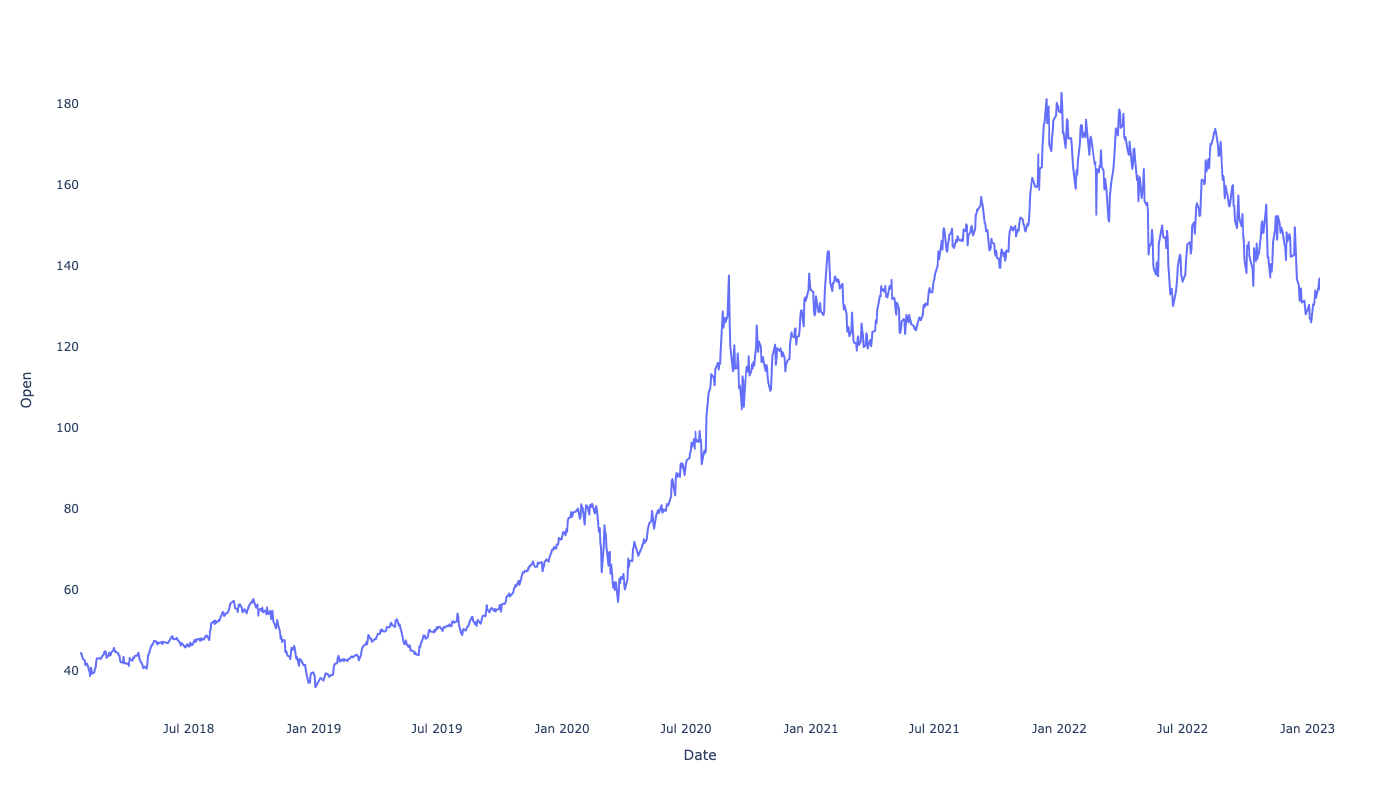
\includegraphics[width=15cm]{open.png}
    \caption{Apple Inc. Open stock price from 2018 to 2023}
    \label{fig:open}
\end{figure}
    \item \textbf{The closing price} is the last price at which it is traded on a stock exchange throughout the course of a trading day. The exchange determines the closing price at the conclusion of trading and is based on the final transaction that occurred during the trading day. It is used to compute the net change and percentage change in the stock's value during the course of the trading day, as well as the value of the stock at the conclusion of the trading day.
    \begin{figure}[!h]
    \centering
    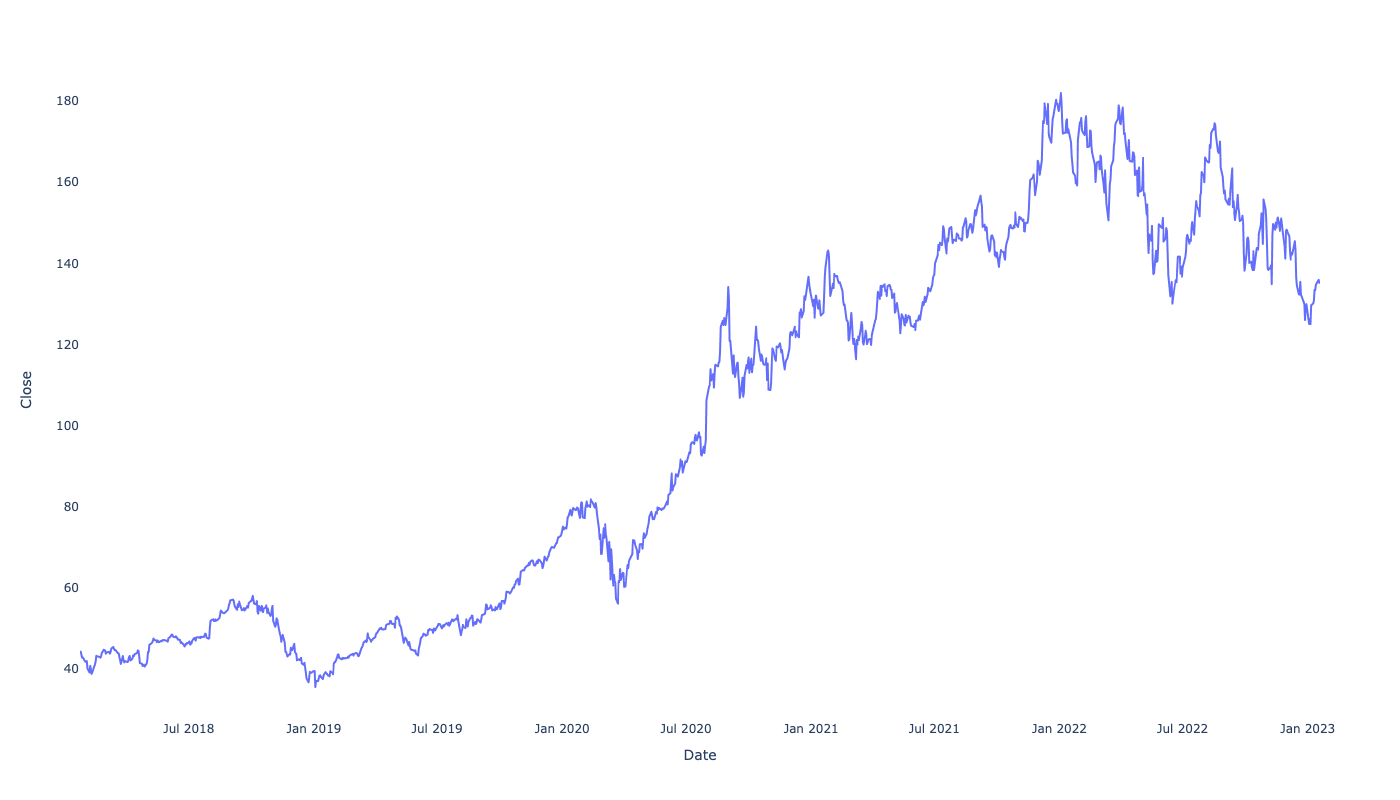
\includegraphics[width=15cm]{close.png}
    \caption{Apple Inc. Close stock price from 2018 to 2023}
    \label{fig:close}
\end{figure}
    \item \textbf{The highest price} at which a stock traded  a certain trading day or period of time is referred to as its high price. It is used to represent the stock's highest price throughout that time period. High prices can help traders, investors, and analysts analyze and make choices about stock performance.
    \begin{figure}[!h]
    \centering
    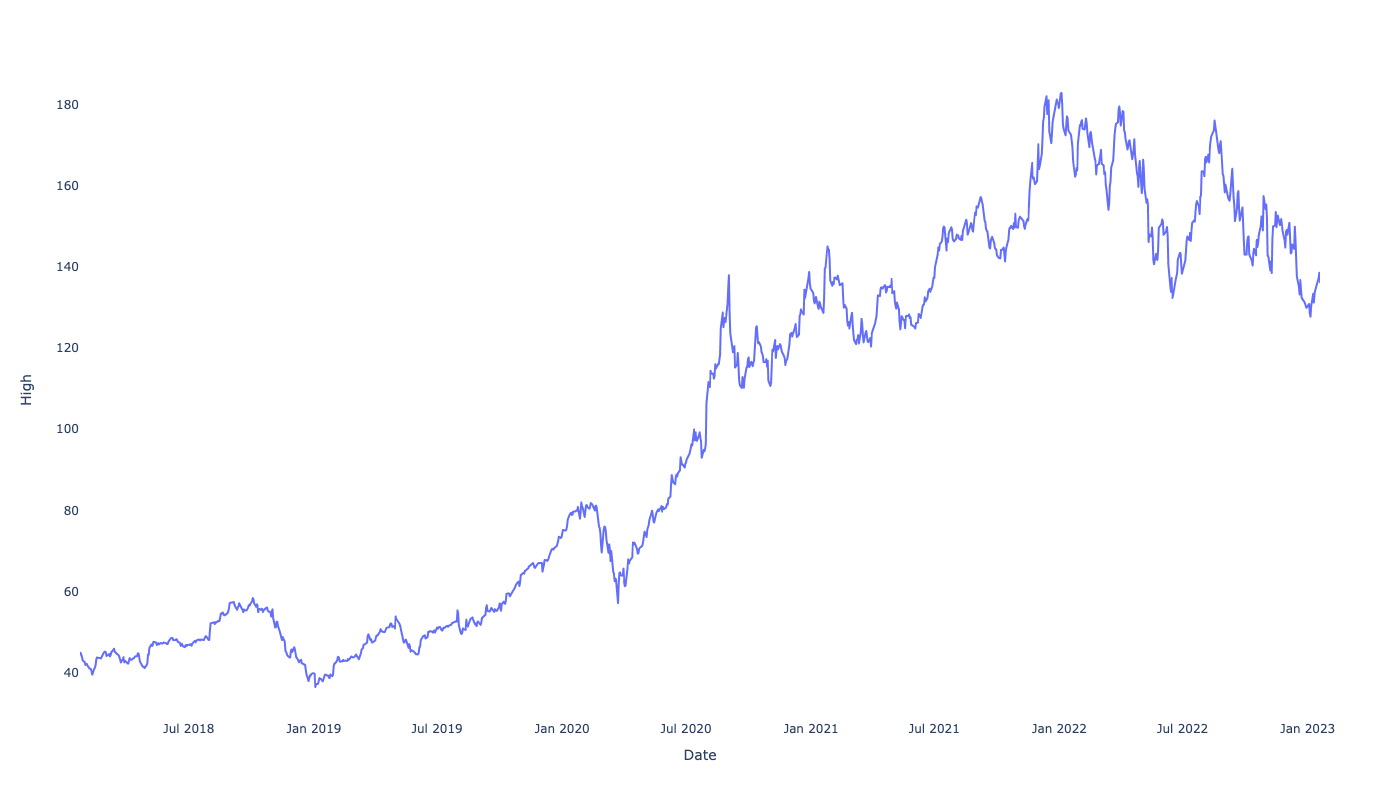
\includegraphics[width=15cm]{high.png}
    \caption{Apple Inc. High stock price from 2018 to 2023}
    \label{fig:high}
\end{figure}
    \item \textbf{The adjusted closing price} of stock takes into account company activities such as stock splits, dividends, and other special events that may affect the stock's price. The adjusted close price is used to calculate a stock's historical return and is said to be a more accurate representation of the stock's performance than the ordinary closing price. This price is used to correct these occurrences and provide a more realistic view of the stock's performance over time.
\begin{figure}[!h]
    \centering
    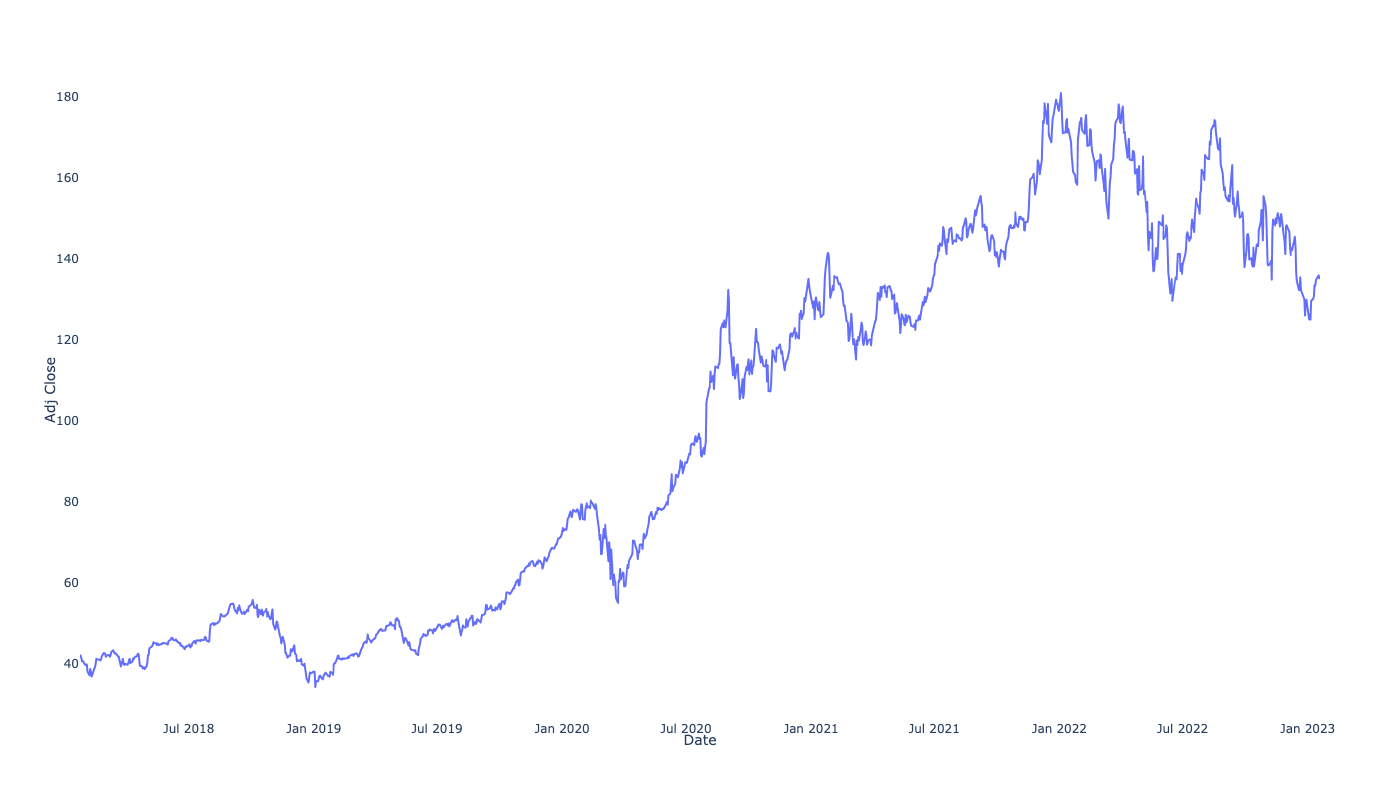
\includegraphics[width=15cm]{adjclose.png}
    \caption{Apple Inc. Adjusted Close stock price from 2018 to 2023}
    \label{fig:adj}
\end{figure}
    \item \textbf{The volume} of stock refers to the number of shares traded during a certain trading day or period of time. It is used to show a stock's degree of activity and liquidity. High volume usually implies a high degree of interest in a stock, whilst low volume may imply a lower level of interest. Stock volume may be a useful statistic for traders, investors, and analysts for evaluating stock performance, making choices, and forecasting future price movements.
    \begin{figure}[!h]
    \centering
    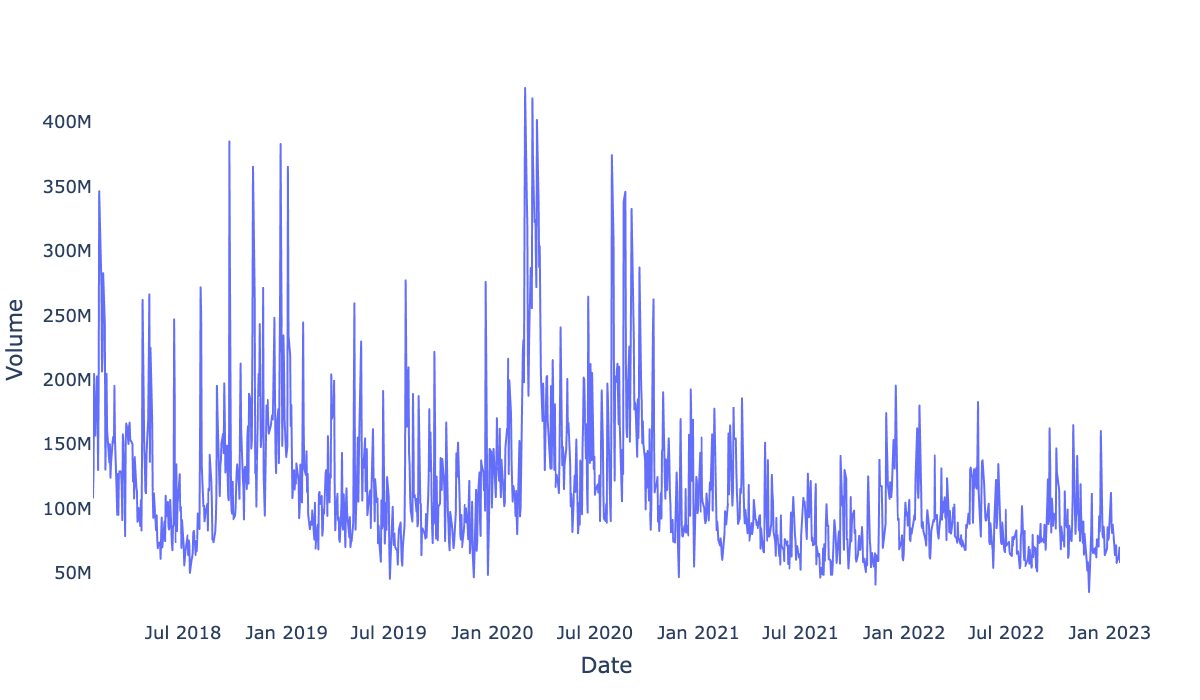
\includegraphics[width=15cm]{vol.png}
    \caption{Apple Inc. stock price volume from 2018 to 2023}
    \label{fig:vol}
\end{figure}
\item \textbf{The low price} is the lowest price that a stock reached during a trading day. It is one of several indicators of a stock's performance, along with the open price, close price, and high price. These prices provide insight into how the stock's value has changed over a specific period of time and can be used to determine the stock's trend during the trading day and its volatility.
\end{itemize}

\begin{figure}[!h]
    \centering
    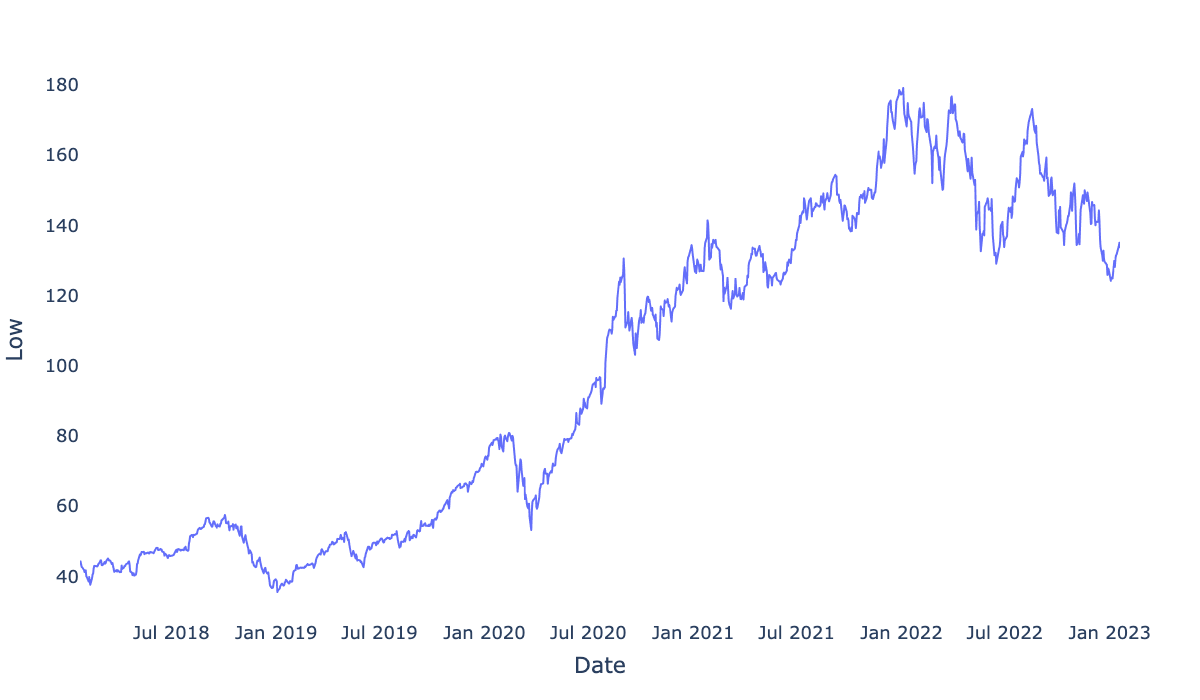
\includegraphics[width=15cm]{low.png}
    \caption{Apple Inc. Low stock price from 2018 to 2023}
    \label{fig:low}
\end{figure}
%%%%%%%%%%%%%%%%%%%%%%%%%%%%%%%%%%%%%%%%%%%%%%%%%%%%%%%%%%%%%%
\subsection{Explanatory Data Analysis}
Exploratory Data Analysis (EDA) is a method for examining and condensing a dataset in order to comprehend its underlying patterns, connections, and structures. Combining visual and statistical techniques, such as producing histograms, scatter plots, and box plots, as well as computing summary statistics like mean, median, and standard deviation, are frequently used to do this. EDA seeks to develop hypotheses about the data and find any potential outliers or abnormalities. It is a crucial first stage in any data analysis project and influences the choice of more sophisticated approaches that may be applied later.

\begin{table}[!h]
    \centering
    \caption{The first ten rows of the Apple stock price dataset.}
    \vspace{5pt}
    \begin{tabular}{|l|l|l|l|l|l|l|}
    \hline
        \textbf{Date} & \textbf{Open} & \textbf{High} & \textbf{Low} & \textbf{Close} & \textbf{Adj Close} & \textbf{Volume} \\ \hline
        2018-01-22 & 44.325001 & 44.445000 & 44.150002 & 44.250000 & 42.077320 & 108434400 \\ \hline
        2018-01-23 & 44.325001 & 44.860001 & 44.205002 & 44.259998 & 42.086819 & 130756400 \\ \hline
        2018-01-24 & 44.312500 & 44.325001 & 43.299999 & 43.555000 & 41.416439 & 204420400 \\ \hline
        2018-01-25 & 43.627499 & 43.737499 & 42.632500 & 42.777500 & 40.677120 & 166116000 \\ \hline
        2018-01-26 & 43.000000 & 43.000000 & 42.514999 & 42.877499 & 40.772205 & 156572000 \\ \hline
        2018-01-29 & 42.540001 & 42.540001 & 41.767502 & 41.990002 & 39.928280 & 202561600 \\ \hline
        2018-01-30 & 41.382500 & 41.842499 & 41.174999 & 41.742500 & 39.692936 & 184192800 \\ \hline
        2018-01-31 & 41.717499 & 42.110001 & 41.625000 & 41.857498 & 39.802284 & 129915600 \\ \hline
        2018-02-01 & 41.792500 & 42.154999 & 41.689999 & 41.945000 & 39.885494 & 188923200 \\ \hline
        2018-02-02 & 41.500000 & 41.700001 & 40.025002 & 40.125000 & 38.154842 & 346375200 \\ \hline
    \end{tabular}
\end{table}
\textbf{Correlation}

We calculate the correlation of the columns with each other, the result of this correlation function is a table showing the correlation between the columns. At a glance, we can see that this has a matrix of size $n \times n $ where $n$ is the number of columns in the table. And the positions on the main diagonal of the matrix represent the correlation of an attribute to itself, so the result of the correlation at the main diagonals on the matrix is 1.

Here we use the Pearson method. Given the paired data $\{(x_1,y_1),...,(x_{n},y_{n})\}$, the Pearson correlation is calculated as follows:

$$
r_{xy} = \frac{\sum_{i=1}^{n}(x_{i}-\Bar{x})(y_{i}-\Bar{y})}{\sqrt{\sum_{i=1}^{n}(x_{i}-\Bar{x})^2}\sqrt{\sum_{i=1}^{n}(y_{i}-\Bar{y})^2}}
$$

where,

\begin{itemize}[leftmargin=7.5pt]
    \item $n$ is the sample size
    \item $x_{i}, y_{i}$ are the individual sample points indexed with $i$
    \item $\bar{x}$ and $\bar{y}$ are, respectively, mean value of $x_i$ and mean value of $y_i$.
\end{itemize}

Pearson correlation coefficient $r_{xy}$ fluctuates in the continuous range from -1 to 1 (i.e. $r_{xy} \in [-1,1]$). Specifically, strong positive relationships are indicated by a coefficient of 1, strong negative relationships are shown by a coefficient of 1, and no linear relationships are indicated by a value of 0. To ascertain the relationship between variables in data analysis, the Pearson correlation is frequently utilized.

    
\begin{figure}[!h]
    \centering
    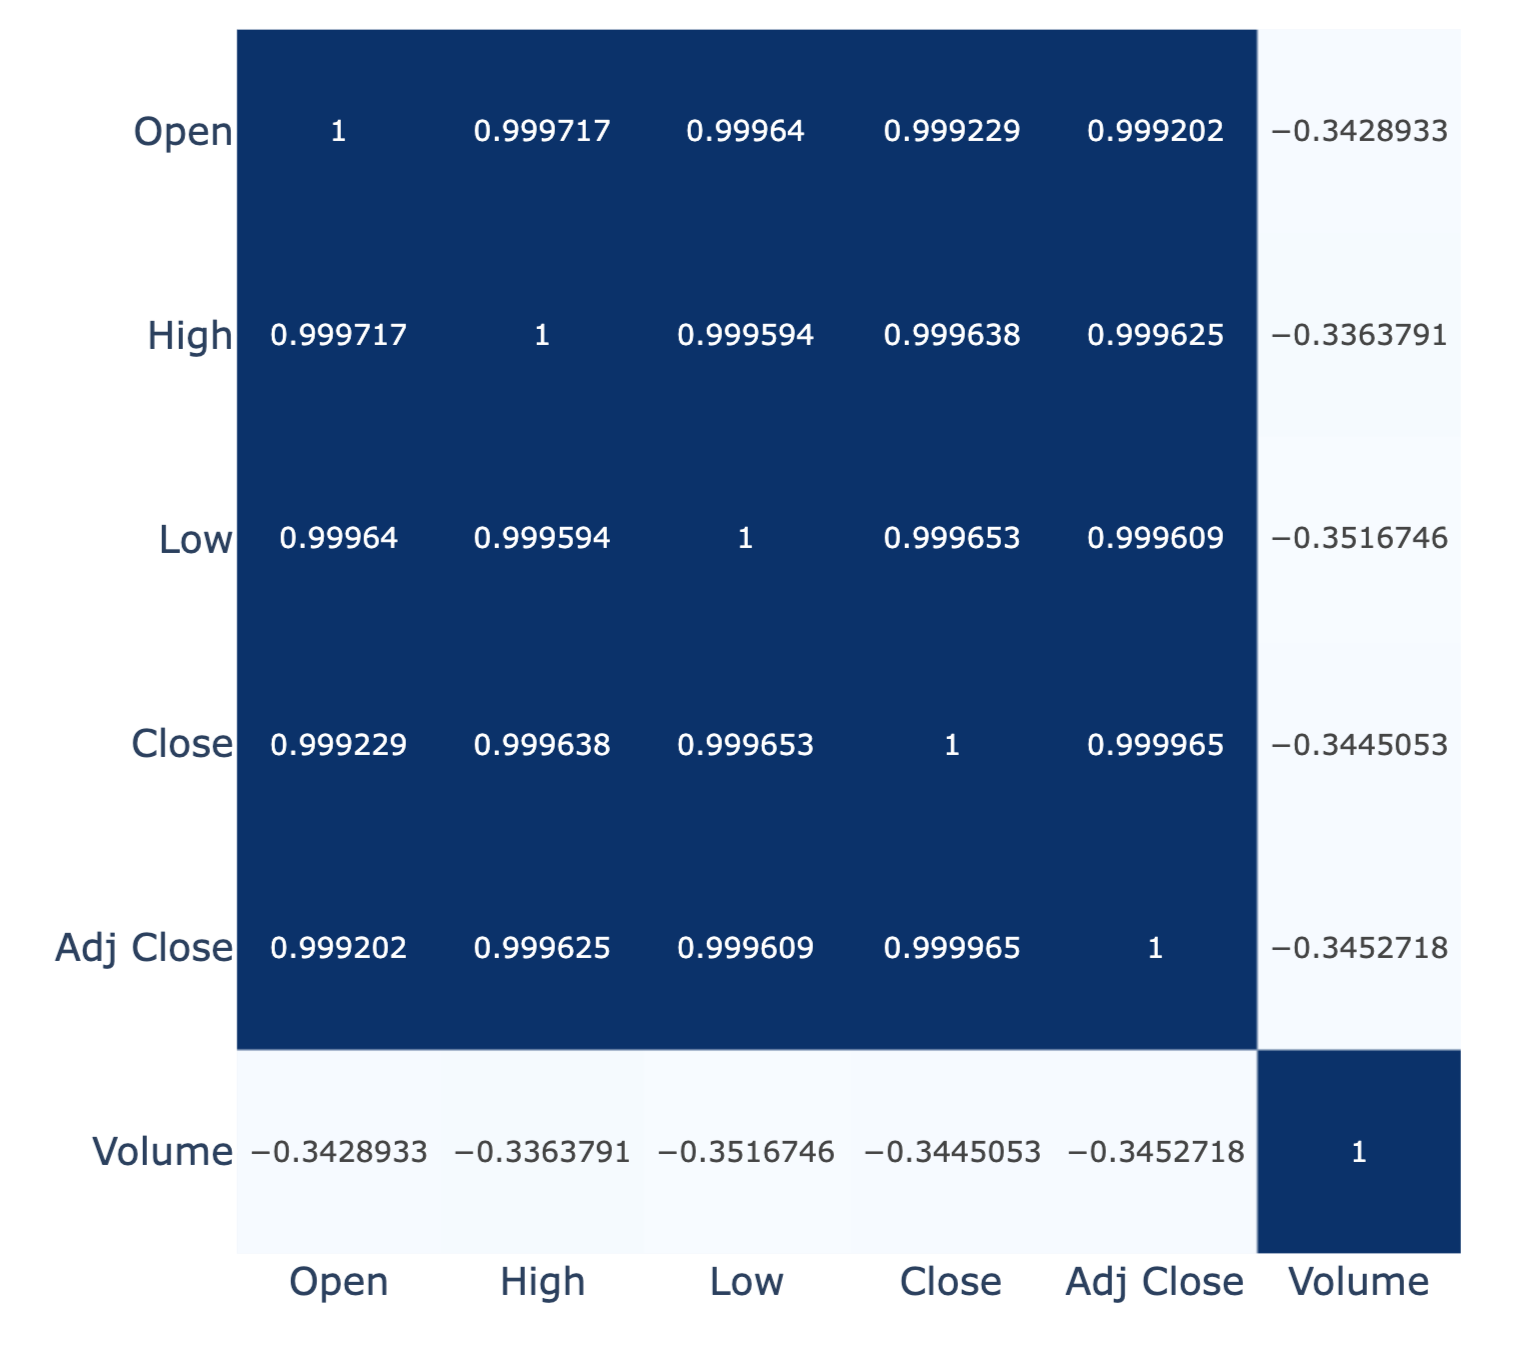
\includegraphics[width=11cm]{corr.png}
    \caption{Correlation heatmap of the dataset}
    \label{fig:corr}
\end{figure}

It is noteworthy that we must choose the $X$ and $y$ of the problem appropriately, as with any supervised learning task on tabular data. Typically, $X$ represents the features and $y$ is the label for the features $X$ (usually clearly defined in the data table). The precise labels provided by the problem are not included in this problem, though. As a result, we must modify the data's input as well as the output using the Sliding Window method (later described in section \ref{window}).

\begin{figure}
    \centering
    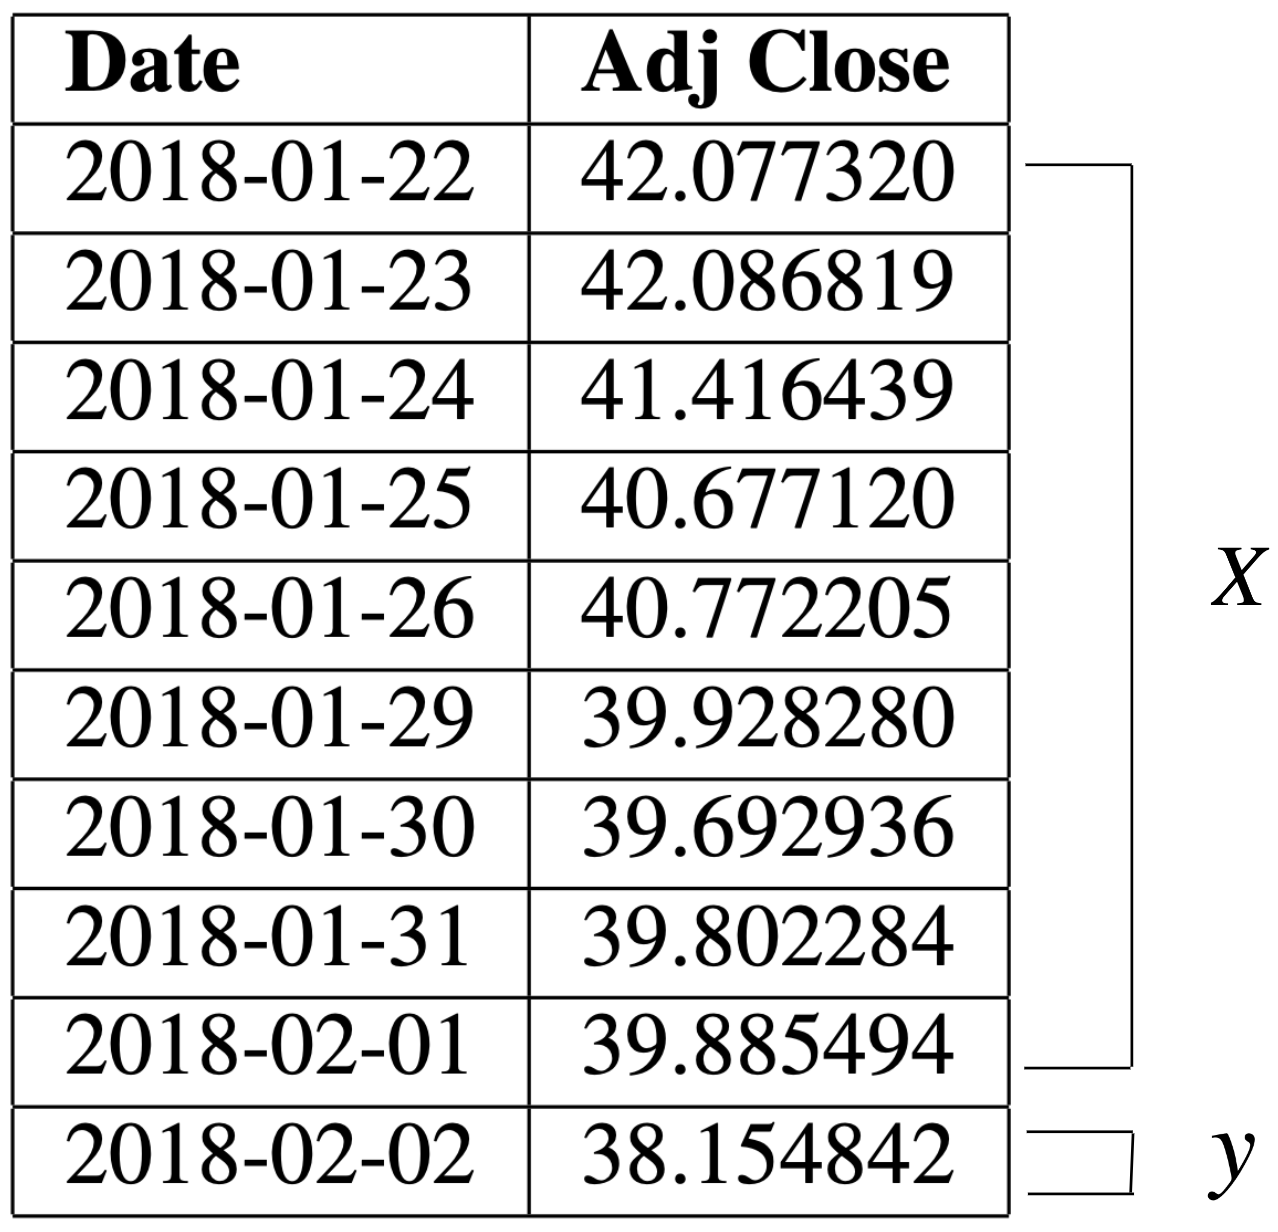
\includegraphics[width=5cm]{target.png}
    \caption{How to determine $X, y$ based on samples of a given data table}
    \label{fig:xy}
\end{figure}

We first look for the relationship between the close price and the adjusted close price. We observe a strong correlation between these two characteristics. This implies that when the closing price rises, so will the adjusted close price. Furthermore, it rises by a nearly identical quantity. It's known as a positive correlation.

We also discover that there is a negative correlation between the volume sold and the adjusted close price. We can thus infer that if the total number of shares sold throughout the day rises, the adjusted close price would fall; nevertheless, there is not a strong association between these two characteristics.

It is important to note that columns: open, close, low, high, adj close, in the dataset have a strong dependency. This dependency reflects in the strong correlation. This matter is easy to understand because they depend on the change in stock price on a trading day. However, the most important variable for stock price prediction is the adjusted close price variable. Therefore, in this work, we will only consider the data of the Adjusted Close Price. Generally speaking, the considered problem is the \textit{univariate regression} of time series.

\textbf{Moving Average}

A statistical technique for analyzing time series data is the moving average. It is an assessment of the typical value of a collection of data points over a certain time frame. Taking the average of a predetermined number of data points, the moving average is created by "pushing" this average ahead by one data point to create the subsequent average. Up until all data points are included in the moving average, this process is repeated.

\begin{figure}[!h]
    \centering
    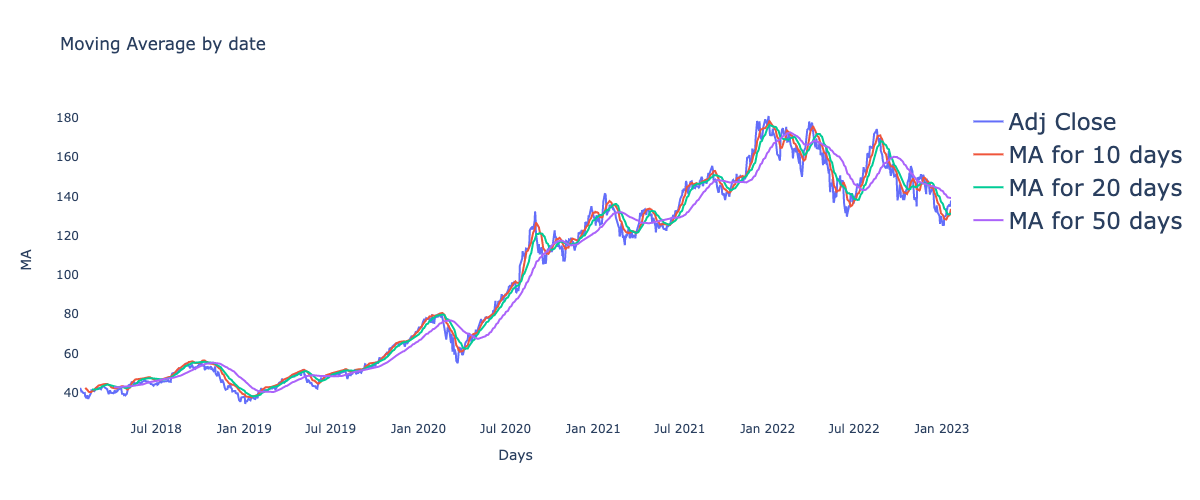
\includegraphics[width=15cm]{ma.png}
    \caption{Moving average on Apple stock price for 10 days, 20 days, 50 days}
    \label{fig:ma}
\end{figure}

Here, we compute the moving average values for the corresponding lengths of 10 days, 20 days, and 50 days as shown in Fig. \ref{fig:ma}. Because a moving average is a broad indication that demonstrates how data is smoothed and utilized to corroborate price patterns, it is of particular relevance to us.
%%%%%%%%%%%%%%%%%%%%%%%%%%%%%%%%%%%%%%%%%%%%%%%%%%%%%%%%%%%%%%
\subsection{Data Normalization}
The practice of putting data values into a consistent scale or distribution is known as data normalization. This is frequently done to ensure that various data characteristics are on a comparable scale, which can increase the accuracy of a prediction model. There are several different types of data normalization that are commonly used in statistics and data analysis. Some of the most common types include:

\textbf{Min-Max Normalization}: This method scales the data so that it falls between a specified range, usually between 0 and 1. The formula for this method is $\frac{x-min}{max-min}$, where $x$ is the initial input, $min$ is the minimum value and $max$ is the maximum value in the dataset.


\textbf{Logarithmic Normalization}: This method scales the data by applying a logarithmic transformation. The formula for this method is $log(x+1)$, where x is the initial input. This method is mostly used for datasets with a skewed distribution where the presence of outliers or extreme values can affect the analysis.

\textbf{Z-Score Normalization} is a way of transforming a variable's values so that they have a mean of zero and a standard deviation of one. This is often done to make sure that different features of the data are on a similar scale, which can help improve the accuracy of a prediction model.

The primary advantage of this approach is that it normalizes the scale of the data, which is beneficial for comparing data and dealing with algorithms that are sensitive to the input scale. This is due to the fact that standardizing the data will make the algorithm less susceptible to the magnitude of the input and, thus, less likely to be influenced by outliers or extreme numbers.

Another advantage of Z-score normalization is that it allows the data to be transformed into a standard normal distribution, which can be useful in certain types of statistical analysis and machine learning models that assume that the data has the normal distribution.

In the case of stock price prediction, Z-score normalization may be applied to historical stock prices and other financial data, such as earnings or revenue, to make sure that these features are all on a similar scale and can be used effectively in a prediction model. 

The formula for this method is $\frac{x-\mu}{\sigma}$, where $x$ is the original value, $\mu$ is the mean and $\sigma$ is the standard deviation of the dataset.  In this work, we normalized the data using this method by default choice of the \hyperlink{https://www.tensorflow.org/api_docs/python/tf/keras/layers/Normalization}{Tensorflow normalization layer}. 
%%%%%%%%%%%%%%%%%%%%%%%%%%%%%%%%%%%%%%%%%%%%%%%%%%%%%%%%%%%%%%
\subsection{Sliding Window method} \label{window}

The sliding window method is a technique used to split a sequence of data, such as a time series or a text, into smaller, overlapping segments called windows. The size of the window, or the number of data points it contains, is a user-specified parameter. Each window is then processed separately, and the results are combined to produce a final output.

For example, in a time series analysis, a window of size 10 may be used to extract features from a sequence of 100 data points. The first window would contain data points 1 through 10, the second window would contain data points 2 through 11, and so on. This process continues until the final window, which contains data points 91 through 100.

In text processing, a window of size 2 may be used to extract sequences of words called n-grams. The first window would contain the first and second words, the second window would contain the second and third words, and so on.

The overlapping nature of the sliding window method allows for the capture of temporal or sequential dependencies between data points. It is commonly used in signal processing, natural language processing, and other fields where sequential data is analyzed.

The sliding window method can also be applied to forecast stock prices. In this application, historical stock price data is split into windows of a user-specified size, and each window is used to train a model to predict the next stock price. The size of the window determines the number of previous stock prices that are used as input to the model.

For example, if a window size of 10 is used, the first window would contain the stock prices from the first 10 days, the second window would contain the stock prices from the second to the eleventh day, and so on. Each window is then used to train a model that predicts the stock price on the 11th day, based on the stock prices from the first 10 days.

The pseudocode of the sliding window method could be expressed as follows:

\begin{figure}[!h]
    \centering
    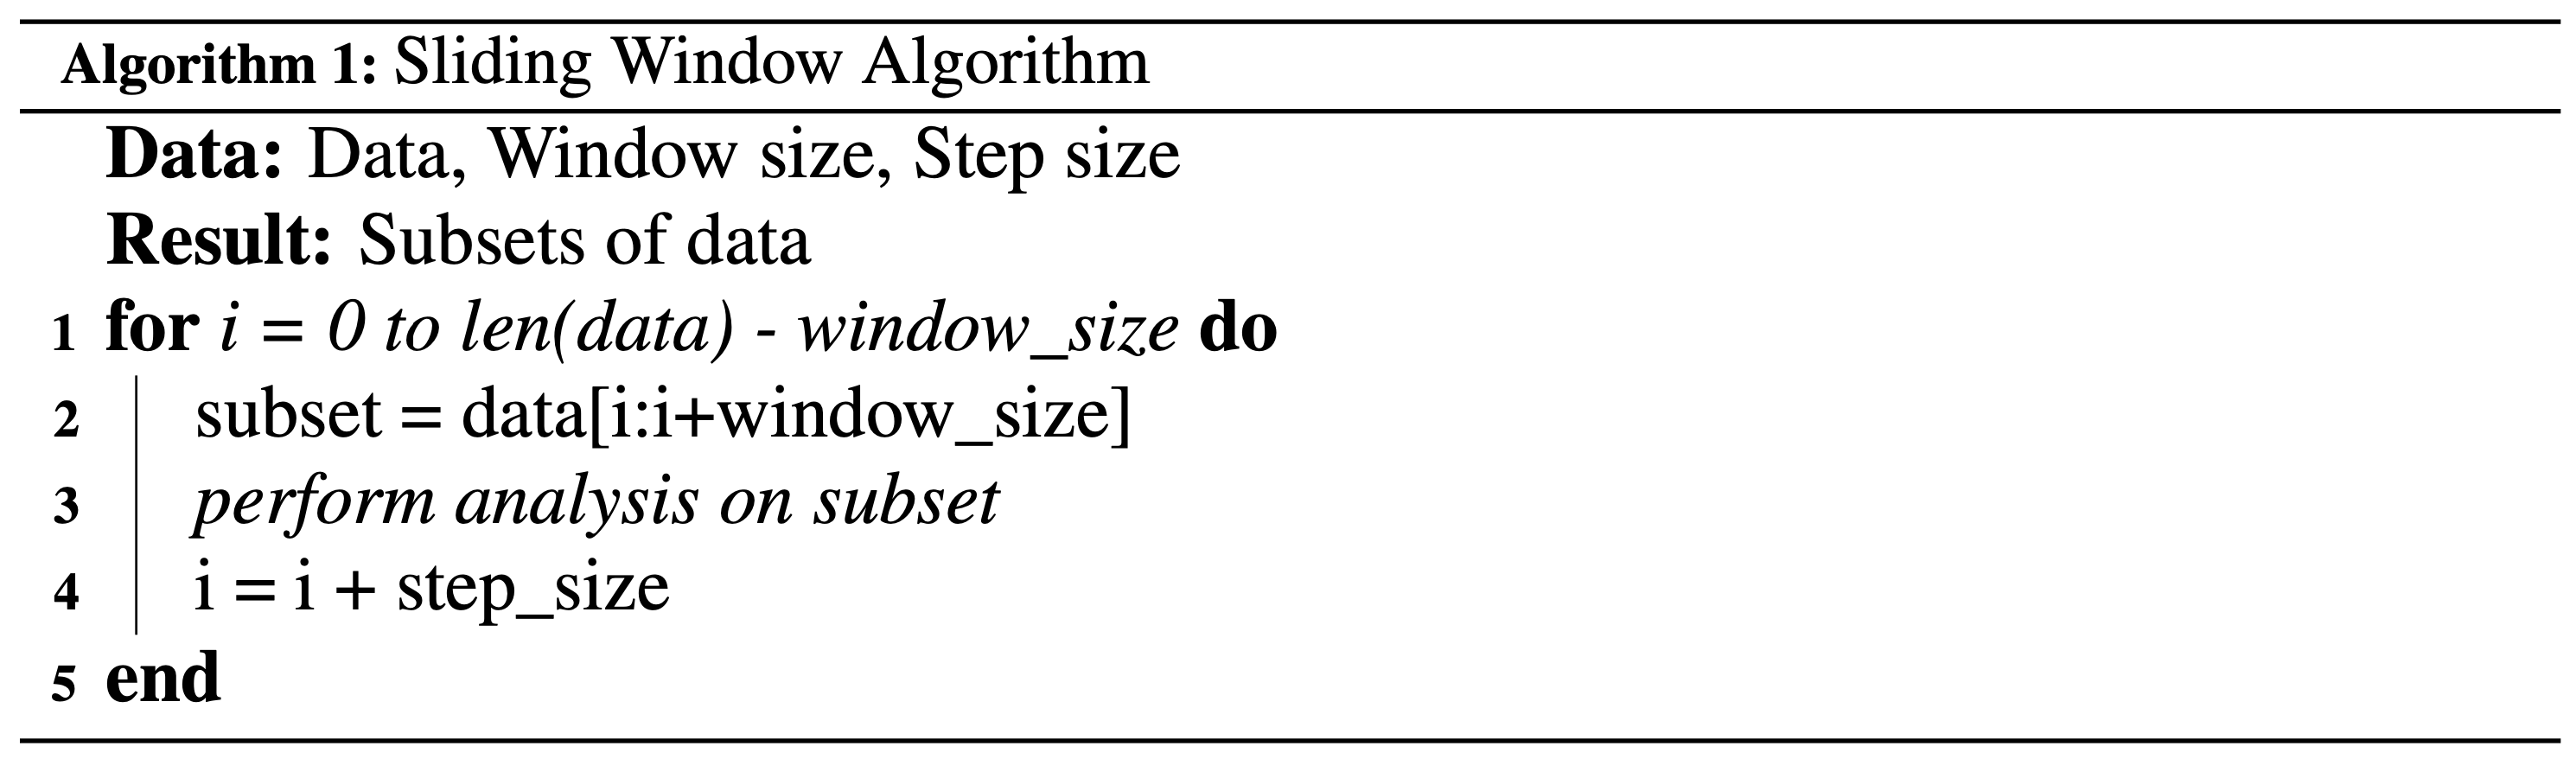
\includegraphics[width=15cm]{windowing.png}
    \caption{Pseudocode of Sliding window algorithm}
    \label{fig:my_label}
\end{figure}

The window size and step size are assumed to be integers, the input is a one-dimensional data array, and the objective is to produce data subsets for examination in this pseudocode. The for loop extracts a portion of the data at each iteration while iterating through the data array by increasing the starting index of the window by the step size. The subset can then be handled any way you'd like.

A final forecast may then be created by combining the models learned on each window. The predictions of all the models can be averaged, or ensemble techniques can be used.
%%%%%%%%%%%%%%%%%%%%%%%%%%%%%%%%%%%%%%%%%%%%%%%%%%%%%%%%%%%%%%%%%%%%%%%%
\section{Model Development}

Model development is the process of building a machine learning model that can predict or decide based on the given data. Problem formulation, data gathering and preprocessing, model selection, model training, model assessment, and model deployment are often included. Before the model performs well enough for deployment, it may need to be modified and re-evaluated several times. This is an iterative process.
%%%%%%%%%%%%%%%%%%%%%%%%%%%%%%%%%%%%%%%%%%%%%%%%%%%%%%%%%%%%%%
\subsection{BiLSTM model for stock price prediction}
Bidirectional Long Short-Term Memory (BiLSTM) [\cite{schuster1997bidirectional}] is a type of Recurrent Neural Network (RNN) [\cite{rumelhart1985learning, jordan1997serial}] which is particularly useful for handling sequential data. BiLSTM is particularly well-suited for stock price prediction because it can remember the historical stock prices for a long time and hence it can be used to predict future prices based on past prices.

BiLSTM is well-suited for time series data and has been applied in many applications, including stock price prediction. The main advantage of BiLSTM over other models, such as traditional feedforward neural networks [\cite{rosenblatt1958perceptron}], is its ability to retain information from previous time steps, which is important in predicting stock prices as the prices are often influenced by historical data.

Additionally, BiLSTM is capable of handling the problem of vanishing gradients, a common problem in conventional RNNs. We describe this problem in section \ref{gradient}. This is because BiLSTM includes a memory cell, input gate, forget gate, and output gate (later described in \ref{lstm architecture}), which allow it to selectively store, update, and access information from previous time steps. This enables the model to make more accurate predictions as it can take into account long-term dependencies in the data.

The choice of using a BiLSTM model for stock price prediction is based on the unique properties of this type of model and its ability to effectively learn from time series data. This is thanks to the following properties:

\textbf{Handling temporal dependencies:} BiLSTM is particularly well-suited for handling temporal dependencies, which are present in many time series datasets, including stock prices. This is due to the fact that BiLSTM has a "memory" component that can remember past information, allowing the model to effectively capture long-term dependencies in the data.

\textbf{Handling noise:} BiLSTM is able to handle noise in time series data, which is also a common problem when working with stock price data since BiLSTM has a "memory" component that can remember past information, allowing the model to effectively capture the underlying patterns in the data despite the presence of noise.

\textbf{Handling non-linearity:} BiLSTM is able to handle non-linearity in time series data, which is a common problem when working with stock price data due to the fact that BiLSTM is a type of neural network that is able to learn non-linear relationships between inputs and outputs.

\textbf{Handling of multi-dimensional data:} Stock prices are under influence of a variety of factors, such as economic indicators, news articles, and social media sentiment. BiLSTM can handle high-dimensional data and can be used with multiple input and output layers, which allows them to process and make predictions based on multiple types of data.

There are a variety of models that can be used for stock price prediction, including ARIMA, GARCH, and deep learning models such as CNNs and Autoencoders. 

\textbf{ARIMA (Auto-Regressive Integrated Moving Average)} is a time series forecasting model that assumes a time series' future value is a linear function of its previous values and mistakes. ARIMA models are commonly used in banking, although they cannot capture non-linear connections in data, which limits their effectiveness.

\textbf{GARCH (Generalized Autoregressive Conditional Heteroscedasticity)} models are employed to represent volatility in financial time series data. While GARCH models may capture stock price inconsistency, they can not account for other variables that influence stock prices.

\textbf{CNNs (Convolutional Neural Networks) and Autoencoders} are deep learning models that have been used for stock price prediction. CNNs are particularly well-suited for computer vision tasks, and they can be used to extract features from financial data such as stock charts. Autoencoders are another type of unsupervised learning that can be used to extract features from the data and to identify patterns in the data.

BiLSTM can more successfully capture the long-term relationships and patterns in financial time series data, giving it an edge over existing models for stock price prediction. Sequential data, long-term dependencies, multidimensional data, noise, and overfitting may all be handled by it. Furthermore, BiLSTM has the capacity to analyze sequential input and preserve an internal memory state, enabling them to preserve context across time, which is crucial for stock price prediction. BiLSTM may thus be superior to other models for the aforementioned causes.
%%%%%%%%%%%%%%%%%%%%%%%%%%%%%%%%%%%%%%%%%%%%%%%%%%%%%%%%%%%%%%
\subsection{Activation functions}

Activation functions are mathematical procedures that are applied to a neuron's output in a neural network. They are used to determine a neuron's output, or the signal it delivers to the next layer of the network. \textbf{The Sigmoid function} (described in \ref{sigmoid}), \textbf{the Hyperbolic Tangent (tanh)} (described in section \ref{tanh}) and\textbf{ the Rectified Linear Unit (ReLU)} (described in section \ref{relu}), and function are examples of common activation functions. The activation function used is determined by the unique problem and the desired model properties.
%%%%%%%%%%%%%%%%%%%%%%%%%%%%%%%%%%%%%%%%%%%%%%%%%%%%%%%%%%%%%%
\subsubsection{Sigmoid activation function} \label{sigmoid}

The sigmoid activation function is one of the most popular activation functions in neural networks and other machine learning models. It is a mathematical function that has values ranging between 0 and 1. The sigmoid function can mathematically be defined as:

$$
sigmoid(x) = \frac{1}{1+e^{-x}}
$$

Where x is the input value and $e$ is the mathematical constant. The sigmoid function produces a curve that is S-shaped, with the output value approaching 0 as the input value becomes more negative, and approaching 1 as the input value becomes more positive, as shown in \hyperref[fig:sigmoid]{Fig. 7}.

\begin{center}
\begin{figure}[!h]
\centering
\begin{tikzpicture}[scale=0.7]
\begin{axis}[
    axis lines = left,
    xlabel = $x$,
    ylabel = {$\frac{1}{1 + e^{-x}}$},
    ymin=0, ymax=1,
    xmin=-6, xmax=6,
    samples=100,
    domain=-6:6,
    smooth
]
\addplot[blue, thick] {1/(1+exp(-x))};
\end{axis}
\end{tikzpicture}
\caption{Sigmoid function plot}
\label{fig:sigmoid}
\end{figure}
\end{center}

When attempting to forecast one of two classes in binary classification issues, the sigmoid activation function is frequently utilized in the output layer of a neural network. The sigmoid function's output may be thought of as a probability, with near values of 0 denoting a low likelihood of the positive class and close values of 1 denoting a high chance of the positive class.

The sigmoid activation function has several advantages, including:

It is differentiable, which allows for the use of gradient-based optimization algorithms for training the neural network.
It outputs values between 0 and 1, which makes it useful for binary classification problems and probability-based predictions.
It compresses the input values into a relatively small range, which can help to prevent the vanishing gradient problem during training.

However, the sigmoid activation function also has some limitations, including:

\begin{itemize}[leftmargin=7.5pt]
    \item It can produce saturating gradients (gradients close to zero) when the input value is far from zero, which can slow down or even stop the training process.
    \item It is not zero-centered, which can cause issues with certain types of initialization and optimization algorithms.
    \item It can produce output values that are not well-suited for multi-class classification problems.
\end{itemize}
%%%%%%%%%%%%%%%%%%%%%%%%%%%%%%%%%%%%%%%%%%%%%%%%%%%%%%%%%%%%%%

\subsubsection{Hyperbolic tangent (Tanh) activation function} \label{tanh}

The Tanh activation function is a popular option for LSTM networks and other neural network architectures. It is a function that maps its input into a number between -1 and 1, in other words, $tanh(x) \in [-1;1]$

The tanh function is defined as:

$$
tanh(x) = \frac{e^x-e^{-x}}{e^x+e^{-x}}
$$

It is equivalent to the logistic sigmoid function, but it is shifted and scaled such that its range is between -1 and 1. This allows for more flexibility in the output of the function, making it a good choice for tasks such as stock price prediction where the output values can vary over a wide range.

\begin{figure}[!h]
\centering
\begin{tikzpicture}[scale=0.7]
\begin{axis}[
    axis lines = left,
    xlabel = $x$,
    ylabel = {$\frac{e^x - e^{-x}}{e^x + e^{-x}}$},
    ymin=-1, ymax=1,
    xmin=-6, xmax=6,
    samples=100,
    domain=-6:6,
    smooth
]
\addplot[blue, thick] {(exp(x) - exp(-x))/(exp(x) + exp(-x))};
\end{axis}
\end{tikzpicture}
\caption{Hyperbolic tangent function plot}
\end{figure}

The tanh function has a number of useful properties. It is a differentiable function, which means that it can be used in backpropagation, a technique used to train neural networks. It is also a monotonically increasing function, which means that it preserves the ordering of its input values. This can be useful in certain types of problems, such as sorting.

The tanh function also has a "centering" effect, where the output values are centered around 0, which can be beneficial for certain types of problems. This is in contrast to the sigmoid function which centers its output around 0.5.

In LSTMs, the tanh function is used as an activation function in the "memory cell" component of the network. The memory cell is responsible for storing the information from previous time steps and passing it along to future time steps. The tanh function is applied to the input to the memory cell, which allows the network to learn which information to keep and which to discard.

The tanh function converts the input into a number between -1 and 1. This is helpful in LSTMs because it enables the network to learn a broad range of values for the information stored in the memory cell, ranging from very negative to extremely positive. This is critical for LSTMs because it enables them to learn to handle a variety of input data types, such as positive and negative numbers. Additionally, the use of the tanh function in LSTMs also provides an additional level of non-linearity, which helps to improve the ability of the network to model complex data.

One limitation of the tanh function is that its output saturates at the extremes, meaning that for large input values, the function's output will be close to 1 or -1, which may cause the gradients to become small and make it difficult for the model to learn.
%%%%%%%%%%%%%%%%%%%%%%%%%%%%%%%%%%%%%%%%%%%%%%%%%%%%%%%%%%%%%%
\subsubsection{ReLU activation function} \label{relu}

The rectified linear unit (ReLU) activation function was originally proposed in the paper "Rectified Linear Units Improve Restricted Boltzmann Machines" by Vinod Nair and Geoffrey Hinton in 2010 [\cite{nair2010rectified}].

In this paper, the authors present an experiment where they trained a deep neural network using the ReLU activation function and compared its performance to networks trained using conventional activation functions such as the sigmoid and hyperbolic tangent. They found that the network trained with the ReLU activation function performed better and was able to converge faster than the other networks.

The authors also showed that ReLU activation functions improve the performance of Restricted Boltzmann Machines (RBMs) as well as Deep Belief Networks (DBNs). The paper also discussed that using ReLU activation functions can be seen as a way of introducing non-linearity in the network.

The paper also discussed that the ReLU activation function is computationally cheaper than other activation functions, making it a more efficient choice for large-scale datasets and deep architectures.

The rectified linear unit (ReLU) activation function is an activation function that is widely used in artificial neural networks. It is defined as $f(x) = max(0,x)$, which means that for any input $x$, the output of the function is either 0 or $x$.

\begin{figure}[!h]
\centering
\begin{tikzpicture}[scale=0.7]
\begin{axis}[
    axis lines = left,
    xlabel = $x$,
    ylabel = {$max(0,x)$},
    ymin=-1, ymax=6,
    xmin=-6, xmax=6,
    samples=100,
    domain=-6:6,
    smooth
]
\addplot[blue, thick, samples=100, domain=-6:6] {(x>0)*x};
\end{axis}
\end{tikzpicture}
\caption{Rectified Linear Unit (ReLU) function plot}
\end{figure}

The ReLU function is a piecewise linear function with a slope of 1 for positive input
values, and a slope of 0 for negative input values. This indicates that while $x$ is positive, the function's output is the same as its input, and when $x$ is negative, the function's output is 0. This is represented graphically as a step function, with the input and output shown on the $x$ and $y$ axes, and the step occurring at $x = 0$. 

The primary advantage of using the ReLU activation function is its computational efficiency. Unlike other activation functions like as sigmoid and tanh, the ReLU function lacks an exponential component, making it computationally less expensive to calculate. 

Another benefit of ReLU is that it eliminates the vanishing gradient issue, which may arise when a network's weights are modified during the training phase. The vanishing gradient issue occurs when the gradient of the activation function gets very small, preventing the network from learning from the input data. ReLU overcomes this issue by using a constant gradient of one for positive input values. 

ReLU is often employed in deep learning architectures including CNNs and Fully Connected Networks (FCNs) since it has been shown to improve network performance and training time.

Later in section \ref{results}, we show that ReLU outperforms both Sigmoid and Tanh activation functions in terms of all performance metrics used.
%%%%%%%%%%%%%%%%%%%%%%%%%%%%%%%%%%%%%%%%%%%%%%%%%%%%%%%%%%%%%%
.
%%%%%%%%%%%%%%%%%%%%%%%%%%%%%%%%%%%%%%%%%%%%%%%%%%%%%%%%%%%%%%
\subsection{Vanishing Gradient} \label{gradient}
The vanishing gradient problem is a common problem that can occur during the process of training deep neural networks. It occurs when the gradients of the weights in the network become extremely small during backpropagation, leading the network to learn very slowly or not at all.

Backpropagation is an algorithm used to train neural networks, it works by propagating the errors from the output layer to the input layer through the network [\cite{rumelhart1985learning}]. During this process, the gradients of the weights are calculated and used to update the weight in order to minimize the error of the network. However, when the gradients are very small they will have a small impact on the weight update, making the training slow or even stop.

In other words, the vanishing gradient problem arises when the gradients are multiplied by the weights themselves and the derivatives of the activation functions during backpropagation. As these gradients flow backward through the network, they can become very small and eventually disappear if the weights are very small or the activation functions have small derivatives.

This problem is particularly pronounced in deep neural networks, where the gradients must flow through many layers before reaching the input layer.  Each time the gradients
flow through a layer, they are multiplied by the weights and the derivatives of the
activation functions. This means that by the time the gradients reach the input layer, they may have become very small and unable to update the weights effectively.

In conclusion, the vanishing gradient problem is a typical issue encountered while training deep neural networks. This issue may be solved by utilizing various activation functions, architectures with skip connections, gradient clipping, weight initialization, and batch normalization.
%%%%%%%%%%%%%%%%%%%%%%%%%%%%%%%%%%%%%%%%%%%%%%%%%%%%%%%%%%%%%%
\subsection{LSTM Architecture} \label{lstm architecture}
The input layer has the responsibility to receive the new input data, which in the case of stock price prediction would typically be historical stock prices, trading volume, and other relevant financial indicators. The input layer can also be augmented with additional features such as technical indicators or economic indicators. $X_t$ is passed through a linear transformation represented by a weight matrix $\mathbf{W}_i$ and a bias vector $b_i$, resulting in a new representation $Z_i = \mathbf{W_i} * X_t + b_i$, where operator $*$ denotes convolution.

The hidden layers are responsible for processing the input data and passing it through the LSTM cells [\cite{hochreiter1997long}]. Typically, there are one or more hidden layers in an LSTM model. each hidden layer $i, \text{where } i = 1, 2, ..., L-1$, contains multiple LSTM cells. Each LSTM cell in the $i^{th}$ layer takes as input the output from the $(i-1)^{th}$ layer and the previous hidden state $h_{t-1}$, and a new hidden state $h_t$ is then generated and output $o_t$. Mathematically, this can be represented as follows:

\textbf{Input gate:}
$$ i_t = \sigma(\mathbf{W}_{i} x_t + \mathbf{W}_{i} h_{t-1} + b_i) $$

\textbf{Forget gate:}
$$ f_t = \sigma(\mathbf{W}_{f} x_t + \mathbf{W}_{fh} h_{t-1} + b_f) $$

\textbf{Output gate:}
$$ o_t = \sigma(\mathbf{W}_{o} x_t + \mathbf{W}_{o} h_{t-1} + b_o) $$

\textbf{Candidate memory cell:}
$$ \tilde{c}_t = tanh(\mathbf{W}_{c} x_t + \mathbf{W}_{c} h_{t-1} + b_c) $$

\textbf{Current memory cell:}
$$ c_t = f_t \odot c_{t-1} + i_t \odot \tilde{c}_t $$

\textbf{Current hidden state:}
$$ h_t = o_t \odot tanh(c_t) $$

where:
\begin{itemize}[leftmargin=7.5pt]
\item $x_t$ is the input at time step $t$
\item $h_t$ is the hidden state at time step $t$
\item $c_t$ is the memory cell at time step $t$
\item $\sigma$ is the Sigmoid activation function
\item $\odot$ is the element-wise product
\item $\mathbf{W}$ are weight matrices
\item $\mathbf{b}$ are bias vectors.
\end{itemize}

A memory cell, an input gate, a forget gate, and an output gate are all included in each LSTM cell. The memory cell is in charge of storing data from earlier time steps. The input gate regulates the flow of data into the memory cell, whereas the forget gate regulates the flow of data out of the memory cell. The output gate regulates the flow of information from the memory cell to the next layer. Specifically:

The forget gate regulates how much of the previous cell state $c_{t-1}$, and hence, how much of the prior data, should be forgotten. The forget gate computes a value between 0 and 1 that is then used to weight the prior cell state using the previous hidden state $h_{t-1}$, current input $x_{t}$, and previous hidden state $h_{t-1}$. Most of the previous cell state should be retained if the value is near to 1, whereas most of the previous cell state should be forgotten if the value is close to 0.

Using the prior hidden state $h_{t-1}$, the current input $x_t$, and a value between 0 and 1, the input gate calculates how much of the new candidate cell state $\tilde{c_t}$ should be added to the current cell state ($c_t$).

Using the previous hidden state $h_{t-1}$, the current input $x_t$, and a value between 0 and 1, the output gate calculates how much of the current cell state $c_t$ should be transmitted to the output $h_t$.

The cell state is the LSTM cell's internal memory. It is computed by first calculating a candidate cell state $\tilde{c_t}$, which is a combination of the current input $x_t$ and the previous hidden state $h_{t-1}$. The current cell state is obtained by adding the element-wise product of the input gate $i_t$ and the candidate cell state $\tilde{c_t}$ to the element-wise product of the forget gate $f_t$ and the previous cell state $c_{t-1}$.

The hidden state is the LSTM cell's output at time step $t$, which is transmitted to the next LSTM cell in the network. It is computed by taking the element-wise product of the output gate $o_t$ and the cell state Sigmoid $c_t$.

The number of neurons in each layer is a hyperparameter that must be calculated by trial and error and research. The number of neurons in each layer is normally dictated by the amount of the input data and the problem's complexity. The number of neurons in the input layer is typically equal to the number of features in the input data, however, the number of neurons in the hidden layers and output layer may be established by experimentation.

\begin{center}
\begin{figure}[!h]
    \centering
    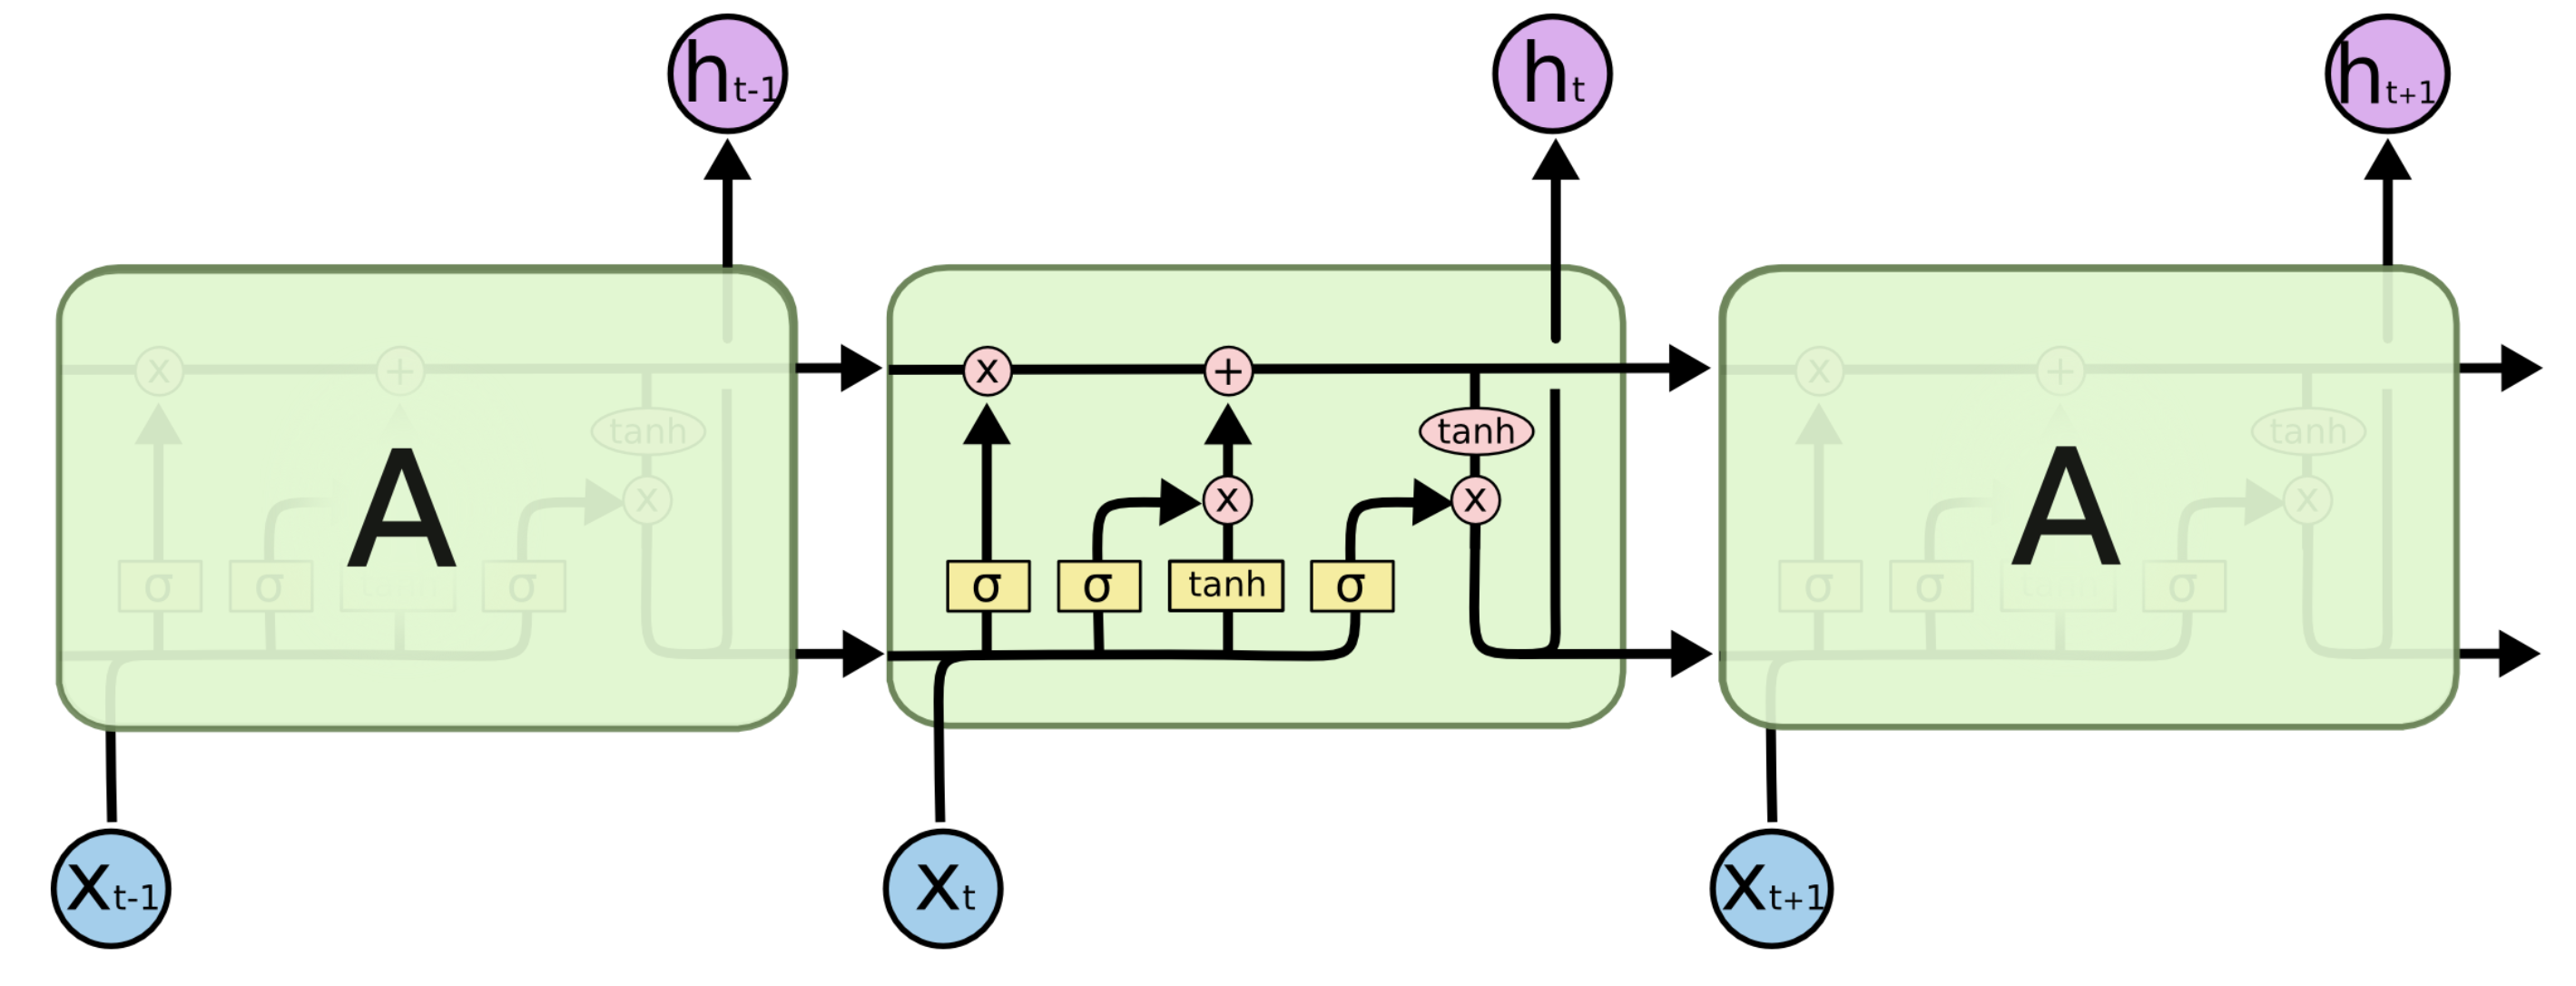
\includegraphics[width=14cm]{lstm.png}
    \caption{LSTM Cell}
    \label{fig:my_label}
\end{figure}
\end{center}

More neurons in the hidden layers, in general, may assist to catch more complicated patterns in data, but it also raises computing needs and the danger of overfitting. As a result, the number of neurons in each layer must be carefully determined, taking into consideration the amount of the input data as well as the problem's complexity. The number of layers in LSTM is likewise a hyperparameter that may be computed in the same manner.
%%%%%%%%%%%%%%%%%%%%%%%%%%%%%%%%%%%%%%%%%%%%%%%%%%%%%%%%%%%%%%
\subsection{Bidirectional LSTM}

The 1997 publication "Bidirectional Recurrent Neural Networks" by \cite{schuster1997bidirectional} is the first one to present the idea of Bidirectional LSTM (BiLSTM).

The BiLSTM architecture was suggested by the authors of the research as a solution to enhance voice recognition tasks. The essential concept underlying the BiLSTM is the employment of two LSTM networks, one moving ahead and the other moving backward. While the backward-facing LSTM reads the input sequence from right to left, the forward-facing LSTM reads it from left to right. The BiLSTM can make predictions by combining the output of the two LSTMs, which allows it to include both past and future contexts.

By feeding past stock market data into the BiLSTM network as input, the same principle of BiLSTM may be used to perform stock price prediction tasks.

First, preprocessed historical stock market data is gathered, including stock prices, trade volume, and other financial indicators. After the stage of data preprocessing, the BiLSTM network then analyzes the preprocessed data in both forward and backward directions, accounting for both historical and recent data to extract meaningful features. While the backward-facing LSTM receives the input sequence from right to left, the forward-facing LSTM reads it from left to right.

The final hidden states of the forward-facing and backward-facing LSTMs are combined and utilized as the final output of the BiLSTM network after the LSTMs have digested the input data.

The output of the BiLSTM is then routed via a fully - connected layer, which generates a forecast of the stock's future price. Multiple neurons may be included in the fully connected layer, which aids in mapping the output from the LSTM to the final prediction.
%%%%%%%%%%%%%%%%%%%%%%%%%%%%%%%%%%%%%%%%%%%%%%%%%%%%%%%%%%%%%%
\subsection{Experiment}
An experiment in stock price prediction using LSTM would involve collecting historical stock price data and any other relevant data, preprocessing the data, splitting the data into training, validation, and testing sets, designing the LSTM model by choosing the appropriate architecture and parameters, training the model on the training set, fine-tuning the model using the validation set and evaluating the model’s performance on the testing set.
%%%%%%%%%%%%%%%%%%%%%%%%%%%%%%%%%%%%%%%%%%%%%%%%%%%%%%%%%%%%%%
\subsubsection{Glorot Uniform Initialization}
Glorot uniform initialization or Xavier uniform initialization is a method for initializing the weights of a neural network, particularly deep neural networks such as LSTM networks proposed by \cite{glorot2010understanding} . It's designed to prevent the vanishing as well as exploding gradients problem by initializing the weights in such a way that the variance of the outputs of each layer is the same as the variance of its inputs, regardless of the number of incoming or outgoing connections.

Mathematically, the Glorot uniform initialization can be defined as:

$$W = \text{Uniform}(-\sqrt{\frac{6}{n_{in} + n_{out}}},\sqrt{\frac{6}{n_{in} + n_{out}}})$$

where $\mathbf{W}$ is the weight matrix, $n_{in}$ is the number of input units, and $n_{out}$ is the number of output units.

This initialization method randomly samples the weights that are uniformly distributed between -$\sqrt{\frac{6}{n_{in} + n_{out}}}$ and $\sqrt{\frac{6}{n_{in} + n_{out}}}$ . By doing this, it ensures that the variance of the output of each neuron is the same as the variance of its inputs and this helps to prevent the vanishing or exploding gradients problem.
%%%%%%%%%%%%%%%%%%%%%%%%%%%%%%%%%%%%%%%%%%%%%%%%%%%%%%%%%%%%%%
\subsubsection{Adaptive Moment Estimation (Adam) Optimization}
Adam (Adaptive Moment Estimation)  is a popular optimization algorithm used to train deep learning models proposed by \cite{kingma2014adam}. It is an extension of the stochastic gradient descent (SGD) algorithm that uses a combination of gradient information and moving averages to adapt the learning rate on a per-parameter basis.

Adam works by maintaining an exponentially decaying average of past gradients as well as past squared gradients, which are used to estimate both the first and second moments of the gradients. The algorithm then uses these estimates to adapt the learning rate for each parameter, with larger updates for parameters with lower first moment (mean) and smaller updates for parameters with higher second moment (variance).

The Adam algorithm has several advantages over traditional optimization algorithms such as SGD. One of the main advantages is that it requires less fine-tuning of the learning rate. Adam can also converge faster and be more sensitive to the choice of initial learning rate.

The Adam algorithm is typically used with a particular fixed learning rate and it is a combination of two other optimization algorithms:

\begin{itemize}[leftmargin=7.5pt]
    \item Root Mean Squared Propagation (RMSProp)
    \item Momentum optimization
\end{itemize}

The algorithm has two main hyperparameters:
\begin{itemize}[leftmargin=7.5pt]
    \item learning rate $\alpha$: controls the step size at which the optimizer makes updates to the model's parameters.
    \item The exponential decay rates $\beta_1 \text{and } \beta_2$: These hyperparameters control the relative weighting of the historical gradients and historical squared gradients in the overall update.
\end{itemize}

Additionally, Adam is an optimization algorithm that uses gradient information and moving averages to adapt the learning rate on a per-parameter basis. The algorithm is defined by the following update equations for each parameter $\theta$:
\begin{enumerate}[leftmargin=7.5pt]
    \item Initialize the parameter $\theta$ with random values, set the learning rate $\alpha$, the decay rate for the first moment estimate $\beta_1$, and the decay rate for the second moment estimate $\beta_2$.
    \item Initialize the first moment estimate $m$ and the second moment estimate $v$ to zero.
    \item Compute the gradient of the loss function with respect to the parameter $\theta$, denoted as $g$.
    \item Update the first moment estimate m with the following equation:
$$    
m = \beta_1 m + (1-\beta_1) g
$$
    \item Update the second moment estimate v with the following equation:
$$
v = \beta_2 v + (1-\beta_2) g^2
$$
    \item Compute the bias-corrected first-moment estimate:
$$\hat{m} = \frac{m}{1-\beta_1^t}$$
    \item Compute the bias-corrected second-moment estimate:
$$\hat{v} = \frac{v}{1-\beta_2^t}$$
\end{enumerate}

Some of the main advantages of using Adam include:
\begin{itemize}[leftmargin=7.5pt]
    \item \textbf{Adaptive learning rate:} Adam automatically adjusts the learning rate for each parameter, which helps to prevent oscillations and divergence during training.
    \item \textbf{Computationally efficient:} Adam requires less memory and is computationally more efficient than other optimization algorithms like gradient descent with momentum.
    \item \textbf{Robustness:} Adam is robust to the choice of the initial learning rate, which makes it easy to use.
    \item \textbf{Combining Momentum and RMSprop:} Adam combine the advantages of both Momentum and RMSprop, which makes it more powerful than either one alone.
    \item Generally it works well with most kinds of Neural Network architectures, with a good trade-off of both speed and quality.
\end{itemize}

The pseudocode of the Adam optimization algorithm could be expressed as follows:

\begin{figure}
    \centering
    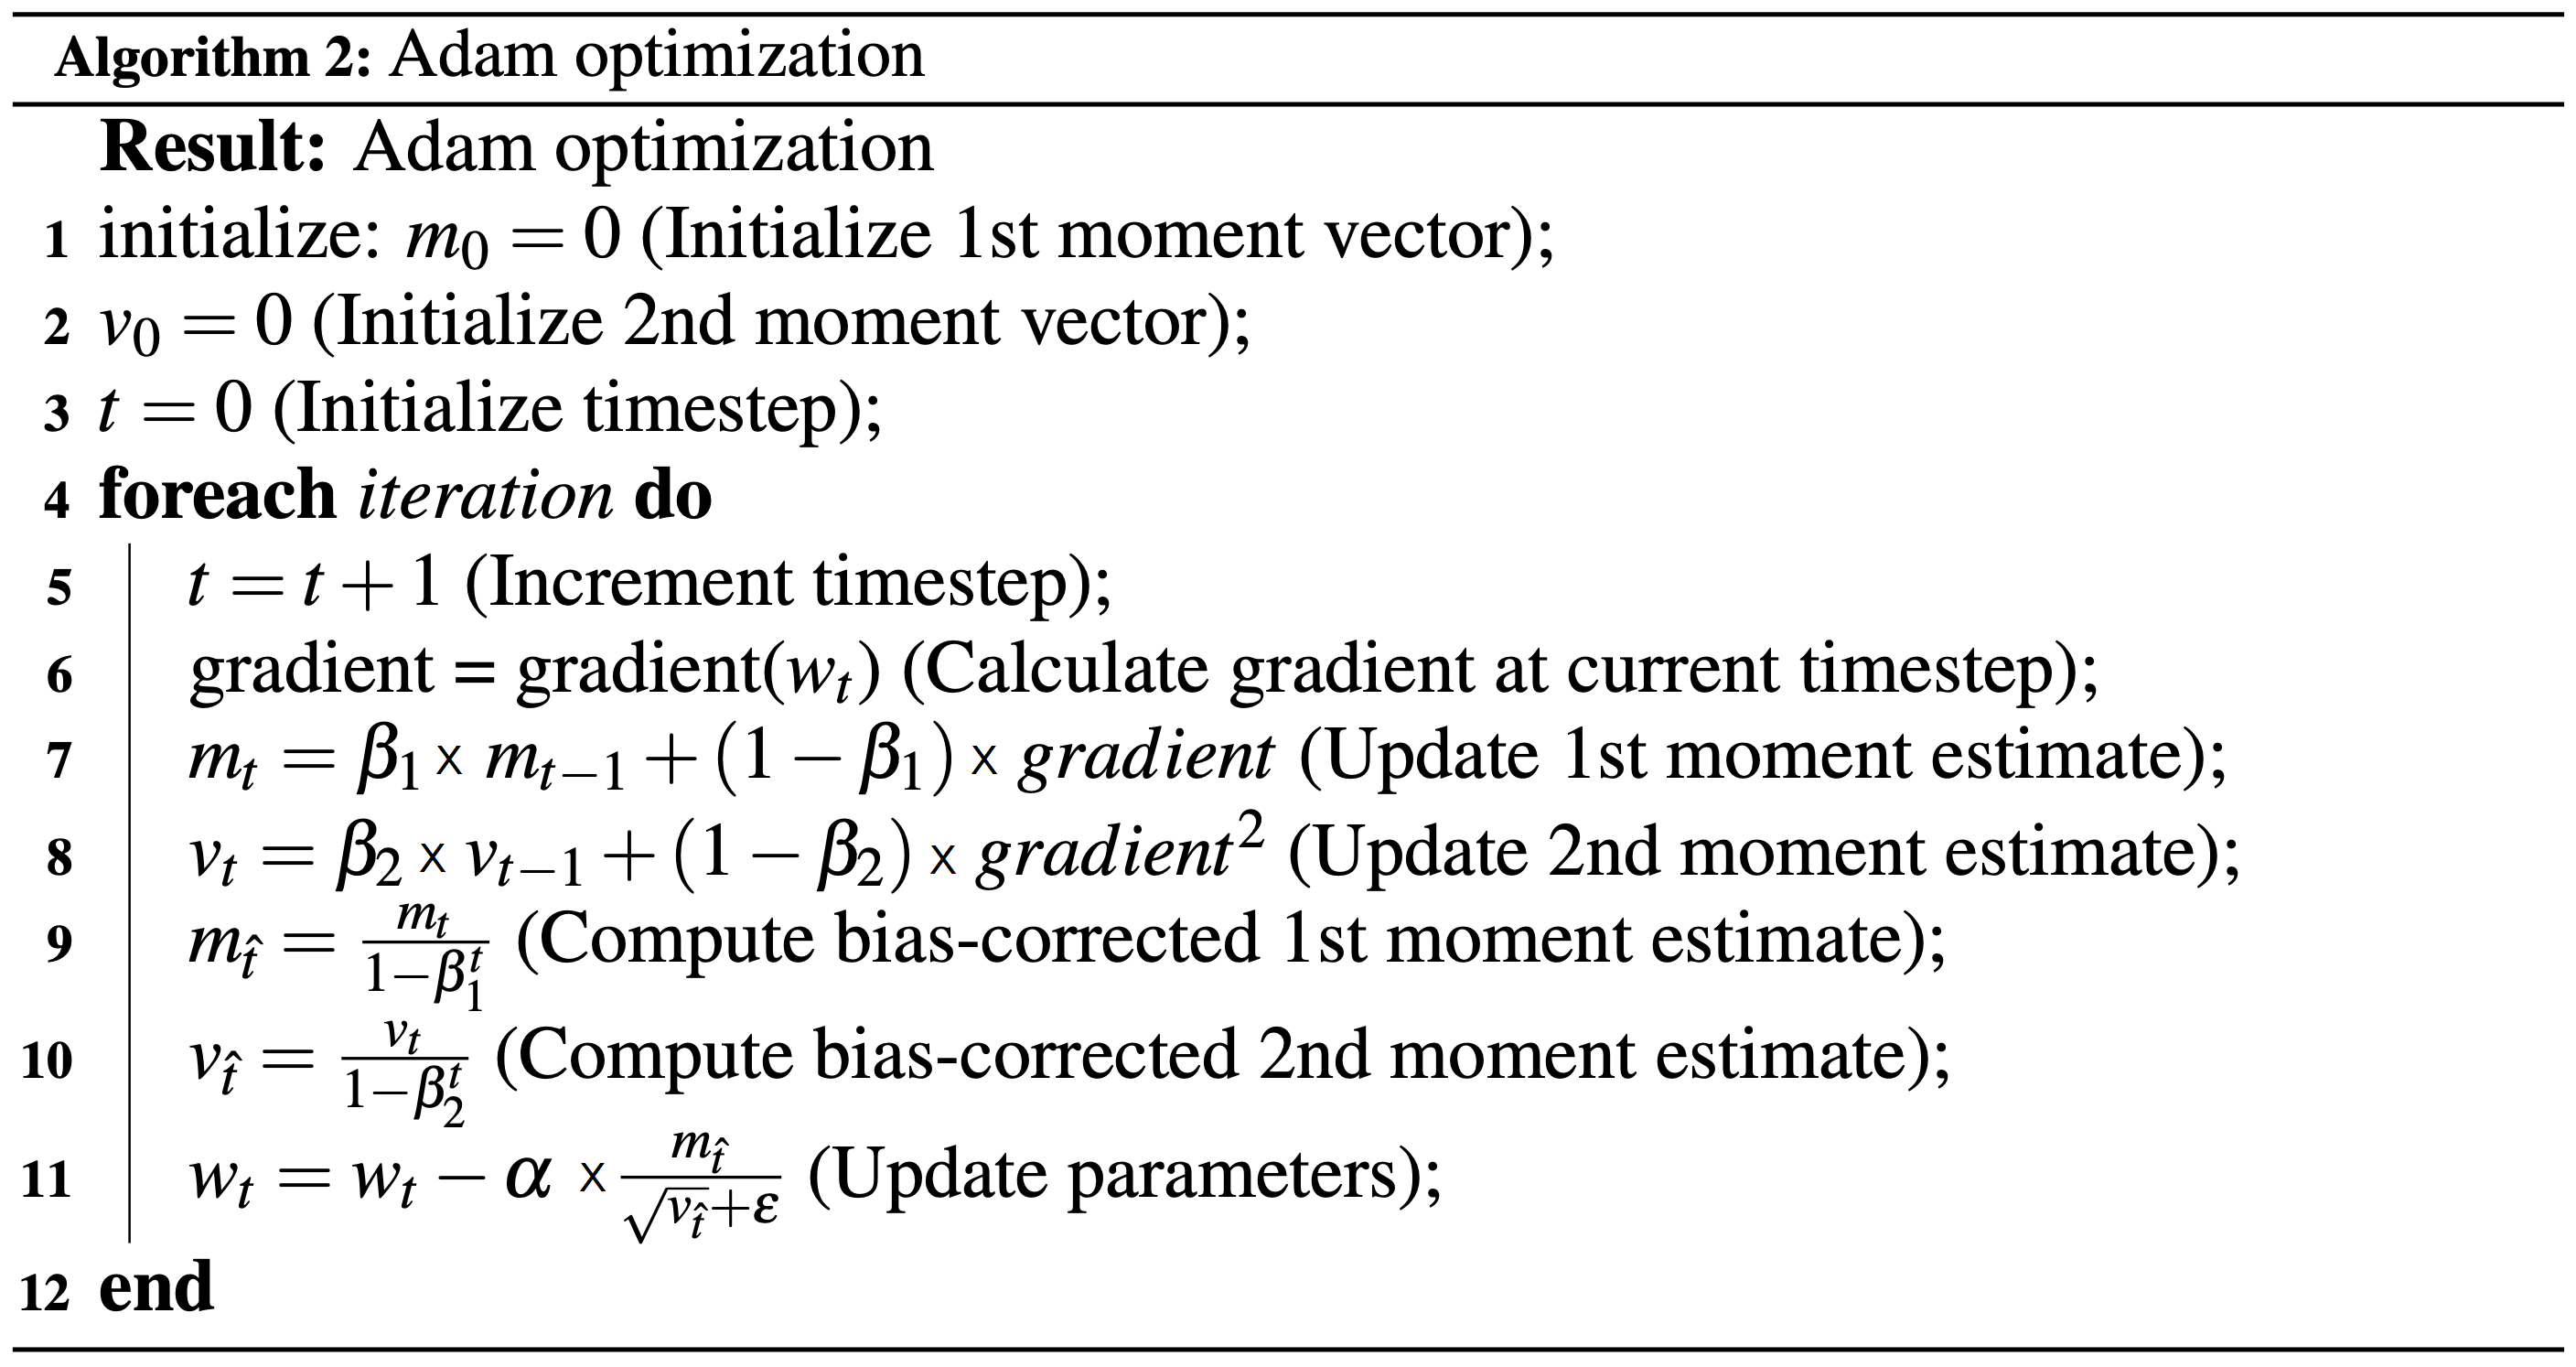
\includegraphics[width=15cm]{adam.png}
    \caption{Pseudocode of Adam optimization algorithm}
    \label{fig:adam}
\end{figure}
%%%%%%%%%%%%%%%%%%%%%%%%%%%%%%%%%%%%%%%%%%%%%%%%%%%%%%%%%%%%%%
\subsubsection{Training Process}

Training a BiLSTM to predict stock prices involves several steps:

\textbf{Data collection:} Collect historical stock market data, including the stock's opening and closing prices, trading volume, and other relevant indicators. In this work, we collect data from Yahoo Finance, a website that keeps records of multiple companies' stock prices. The data used is that of Apple's stock prices from 2018 to 2023.

\textbf{Data preprocessing:} Prepare the data for input into the BiLSTM model. This may include normalizing the data, removing any missing values, and creating a time series dataset by converting the data into sequences of a fixed length. We applied the Z-score normalization method to our dataset via a normalization layer.

\textbf{Model architecture:} Design the LSTM model architecture, including the number of LSTM layers, the number of units in each layer, and any other hyperparameters such as the learning rate and batch size.

In this work, we implement a BiLSTM model that has an architecture as shown in \hyperref[fig:architecture]{Fig. 11}. Specifically:

\begin{figure}[!h]
    \centering
    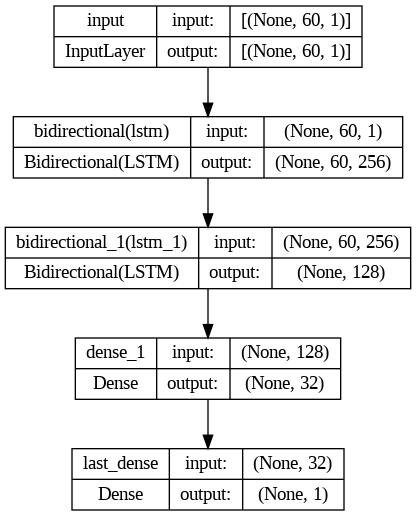
\includegraphics[width=9cm]{architecture.png}
    \caption{BiLSTM Architecture}
    \label{fig:architecture}
\end{figure}

The model architecture is comprised of the following layers:

I\textbf{nput Layer:} This layer defines the shape of the input. The input is expected to be a 2-dimensional tensor with the shape \texttt{(number of samples, number of features, 1)}. The input layer is defined using the Input class in the Keras API and is named "input".

\textbf{Bidirectional LSTM Layer 1:} This is the first LSTM layer in the model and it is bidirectional, meaning it processes the input data in both forward and backward directions. The LSTM layer has 128 units, and the \texttt{return\_sequences} parameter is set to True, meaning that the LSTM layer will output a sequence rather than a single vector. The \texttt{kernel\_initializer} is set to \texttt{tf.initializers.GlorotUniform} with a seed value equal to \texttt{RANDOM\_SEED}. This ensures that the weights of the layer are initialized with the Glorot uniform initializer and the same values will be used every time the model is run.

\textbf{Bidirectional LSTM Layer 2:} This is the second LSTM layer in the model and it is also bidirectional. The LSTM layer has 64 units, and the \texttt{return\_sequences} parameter is set to False, meaning that the LSTM layer will output a single vector instead of a sequence. The kernel\_initializer is set in the same way as the first LSTM layer.

\textbf{Dense Layer 1:} This is the first dense layer in the model and it has 32 units. The activation function used is the Tanh activation function, which is defined as $f(x) = \frac{e^{x}-e^{x}}{e^{x}+e^{x}}$. This layer is named \texttt{dense\_1}.

\textbf{Output Layer:} This is the last layer in the model and it has a single unit, which means it will produce a scalar output. The layer is named \texttt{last\_dense}.

The model is constructed using the Model class in the Keras API and the inputs and outputs are specified as the input layer and the output layer, respectively. The model is returned from the function and can be used for training and making predictions.

Overall, we designed a time-series prediction task, where the input data is a sequence of values and the goal is to predict a single output value. The use of bidirectional LSTMs, normalization, and fully connected layers helps in the process of feature extraction from the input data and makes the final prediction.

\textbf{Model training:} Train the LSTM model using the preprocessed data and the specified architecture. The model will learn to predict stock prices based on the patterns in the historical data.

\textbf{Model evaluation:} Evaluate the trained model using a separate test dataset and metrics such as mean squared error or mean absolute error.

\textbf{Model tuning:} Based on the evaluation results, tune the model by adjusting the hyperparameters, the architecture, or other aspects of the model to improve performance.

\textbf{Model deployment:} Once the model is trained and tuned, it can be deployed on pragmatic grounds and real-world applications to predict based on new stock market data.
%%%%%%%%%%%%%%%%%%%%%%%%%%%%%%%%%%%%%%%%%%%%%%%%%%%%%%%%%%%%%%%%%%%%%%%%
\section{Model evaluation}

Model evaluation is the process of reviewing a machine learning model's performance by testing it on fresh, previously unknown data. Splitting the data into training and testing sets, using cross-validation, evaluating performance using various performance metrics, creating a confusion matrix, and evaluating the performance of binary classifiers by ROC curve are all common techniques for evaluating models. Model evaluation is an iterative process, and changes to the model may be required until the desired level of performance is attained. In this research, we evaluate our model using six metrics, including MAE, MAPE, MPE, MSE, $R^2$, and RMSE.
%%%%%%%%%%%%%%%%%%%%%%%%%%%%%%%%%%%%%%%%%%%%%%%%%%%%%%%%%%%%%%
\subsection{Performance metrics}
Performance metrics are used to evaluate the effectiveness of a model or system. They are used to compare different models or to track the performance of a single model over time. The main purpose of performance metrics is to provide a quantitative measure of how well a model is performing. They can be used to set goals for model development, track progress, and make adjustments as needed. Performance metrics also play an important role in model selection, as well as in the evaluation of model performance in real-world applications.
%%%%%%%%%%%%%%%%%%%%%%%%%%%%%%%%%%%%%%%%%%%%%%%%%%%%%%%%%%%%%%
\subsubsection{Mean Absolute Error, Mean Absolute Percentage Error and Mean Percentage Error}
\textbf{Mean Absolute Error (MAE)} is a measure of the difference between two continuous variables, often an actual and anticipated value. It is determined by taking the average of the absolute discrepancies between projected and actual values. It is, in other words, the average of the absolute error values.

The formula for MAE is:

$$
MAE = \frac{1}{N} \times \sum_{i=1}^{N}|y_{i}-\hat{y_{i}}|
$$

where:
\begin{itemize}
    \item $N$ is the total number of observations
    \item $y_{i}$ is the actual value for the $i^{th}$ observation
    \item $\hat{y_{i}}$ is the predicted value for the $i^{th}$ observation
\end{itemize}

The absolute error values are used in the calculation to ensure that negative and positive differences are treated equally. The use of absolute error values also means that MAE is not affected by the direction of the error (i.e. whether the predicted value is greater or less than the actual value).

MAE is a commonly used metric for evaluating the performance of regression models, as it provides a simple and interpretable measure of the average error. However, it is sensitive to outliers and can be affected by the scale of the data.

\textbf{Mean Absolute Percentage Error (MAPE)}. The Mean Absolute Percentage Error (MAPE) metric is typically used to evaluate the performance of a model when the data has a consistent scale and the percentage of difference matters more than the absolute difference. The MAPE could be defined as:

$$
MAPE = \frac{1}{N} \times \sum_{i=1}^{N}{\frac{|y_{i}-\hat{y_{i}}|}{y_{i}}}
$$

The average of the absolute percentage deviations between the anticipated and actual values is used to determine the MAPE. It is simple to comprehend because it is given as a percentage. Higher MAPE values signify that the model is producing worse predictions, whereas lower MAPE values signify that the model is producing better predictions.


\textbf{Mean Percentage Error (MPE)}. Another metric that we use in this work to measure the model's performance is Mean Percentage Error (MPE). The MPE, in statistics, is the calculated average of the percentage errors by which a model's predictions deviate from the actual values of the quantity predicted. Its mathematical derivation is as follows:

$$
MPE = \frac{1}{N} \times \sum_{i=1}^{N}{\frac{y_{i}-\hat{y_{i}}}{y_{i}}}
$$

Positive and negative forecast mistakes can cancel each other out since the formula uses actual values of the forecast errors rather than their absolute values, which allows it to be used as a metric of forecast bias.

MPE of 0\% means that the predictions of a model are exactly equal to the observed values, while a positive MPE implies that the predictions are overestimating the observed values and a negative MPE means that the predictions are underestimating the observed values.
%%%%%%%%%%%%%%%%%%%%%%%%%%%%%%%%%%%%%%%%%%%%%%%%%%%%%%%%%%%%%%
\subsubsection{Mean Squared Error and Root Mean Squared Error} 
Mean Squared Error (MSE) is a commonly used loss function for regression problems in machine learning and deep learning. It quantifies the mean of the squared differences between the predicted and actual values. The MSE is computed by averaging the squared discrepancies between each data point's expected and actual values. It may be mathematically expressed as:

$$
MSE = \frac{1}{N} \times \sum_{i=1}^{N}(y_{i}-\hat{y_{i}})^2
$$

Where $N$ is the total number of samples in the dataset, $\hat{y_{i}}$ is the predicted values and $y_{i}$ is the actual values. The MSE loss function is differentiable, which means that it can be used with optimization algorithms such as gradient descent to update the model parameters. The MSE is sensitive to outliers, as a single large error can significantly increase the overall MSE.

Mean Squared Error (MSE) has a number of advantages as a loss function. Some of these advantages include:

\textit{Simplicity:} MSE is a straightforward and easy-to-understand measure of a model's ability to predict the target variable given a collection of input variables. Calculated by averaging the squared discrepancies between expected and actual values, it is simple to compute and analyze.

\textit{Differentiability:} The MSE is a differentiable loss function, therefore it may be used with optimization methods like gradient descent to update the model's parameters. The gradient of the MSE loss function with respect to the model's parameters may be determined, and the model's parameters can be modified to reduce the MSE.

\textit{Penalty for large errors:} The MSE is able to penalize large errors more heavily than small errors. This is because the squared difference is used in the calculation of the MSE, which means that large errors will contribute more to the overall MSE than small errors. This can be useful for certain types of problems where large errors are particularly important to avoid.

\textit{Minimization: }MSE can be minimized to find the optimal parameters of the model. Since the MSE is a scalar value, the optimization algorithms can be used to minimize it to find the best parameters that minimize the error.

\textit{Convexity:} The MSE is a convex function, which means that it has only one global minimum. This makes it easier to find the optimal solution.

\textit{Popularity:} MSE is widely used in many machine learning and deep learning algorithms. It is well-understood and has been well-studied, which means that there are many resources available to help practitioners understand and use it effectively.

\textbf{Root Mean Squared Error}. 
The performance of a regression model is also usually measured using the statistic known as Root Mean Squared Error (RMSE). It calculates the differences between actual data and predictions. The RMSE formula could mathematically be derived as:

$$
RMSE = \sqrt{MSE}
$$

The average of the squared differences between the predicted and actual values is used to determine the RMSE. The square root is used to convert the RMSE's units to those of the true and anticipated values.

Because it is simple to comprehend and interpret, the RMSE approach is frequently used to assess a model's performance. Better forecasts are made by the model when the RMSE is lower, and worse predictions are made by the model when the RMSE is larger. 
%%%%%%%%%%%%%%%%%%%%%%%%%%%%%%%%%%%%%%%%%%%%%%%%%%%%%%%%%%%%%%
\subsubsection{$R^2$ score}
In a regression model, the $R^2$ (R-squared) statistic measures the proportion of variance in the dependent variable that can be predicted from the independent variables (also known as predictor or input variables). It evaluates the regression model's compatibility with the data.

The $R^2$ score ranges from 0 to 1, with a value of 1 indicating that the regression line fits the data perfectly and that the independent variables account for all of the variances in the dependent variable. A score of 0 shows that the regression line does not fit the data at all and that the independent variables provide no insight into the dependent variable's variation. In general, a higher $R^2$ value indicates that a larger proportion of the variability in the dependent variable can be explained by the independent variables, suggesting a better fit of the model to the data. The score $R^2$ is computed as follows:

$$
R^2 = 1 - \frac{\sum_{i=1}^{N}{(\hat{y_i}-y_i)^2}}{\sum_{i=1}^{N}{(\bar{y}-y_i)^2}}
$$

where $\bar{y}$ is the mean value.

In conclusion, $R^2$ is a regularly used metric to assess the effectiveness of regression models and it offers a measurement of the model's goodness of fit to the data. An improved model fits the data and a stronger capacity for the independent variables to account for the variability in the dependent variable are both indicated by higher R2 scores.
\subsection{Experimental results and Discussion} \label{results}

The loss of training data is the difference between the expected output and the actual outputs of the model when it is trained on the training dataset. The training data is the subset of the whole dataset that is used to train the model. During the training phase, the model is updated to minimize the loss of the training data. After training the model with 90 epochs using the architecture as described in section \ref{lstm architecture} with Adam optimization method and ReLU activation function, we yield the results as shown in Fig. \ref{fig:loss1} and Fig. \ref{fig:loss2}

\begin{figure}[!h]
    \centering
    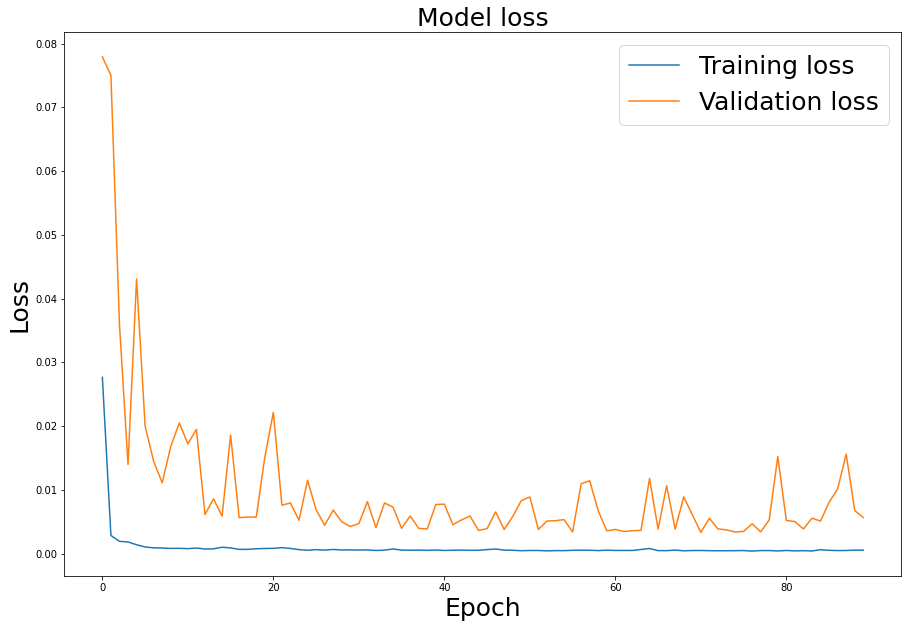
\includegraphics[width=8cm]{r1_1.png}
    \caption{Loss on training data (left) and loss on test data (right) after 90 epochs}
    \label{fig:loss1}
\end{figure}

\begin{figure}[!h]
    \centering
    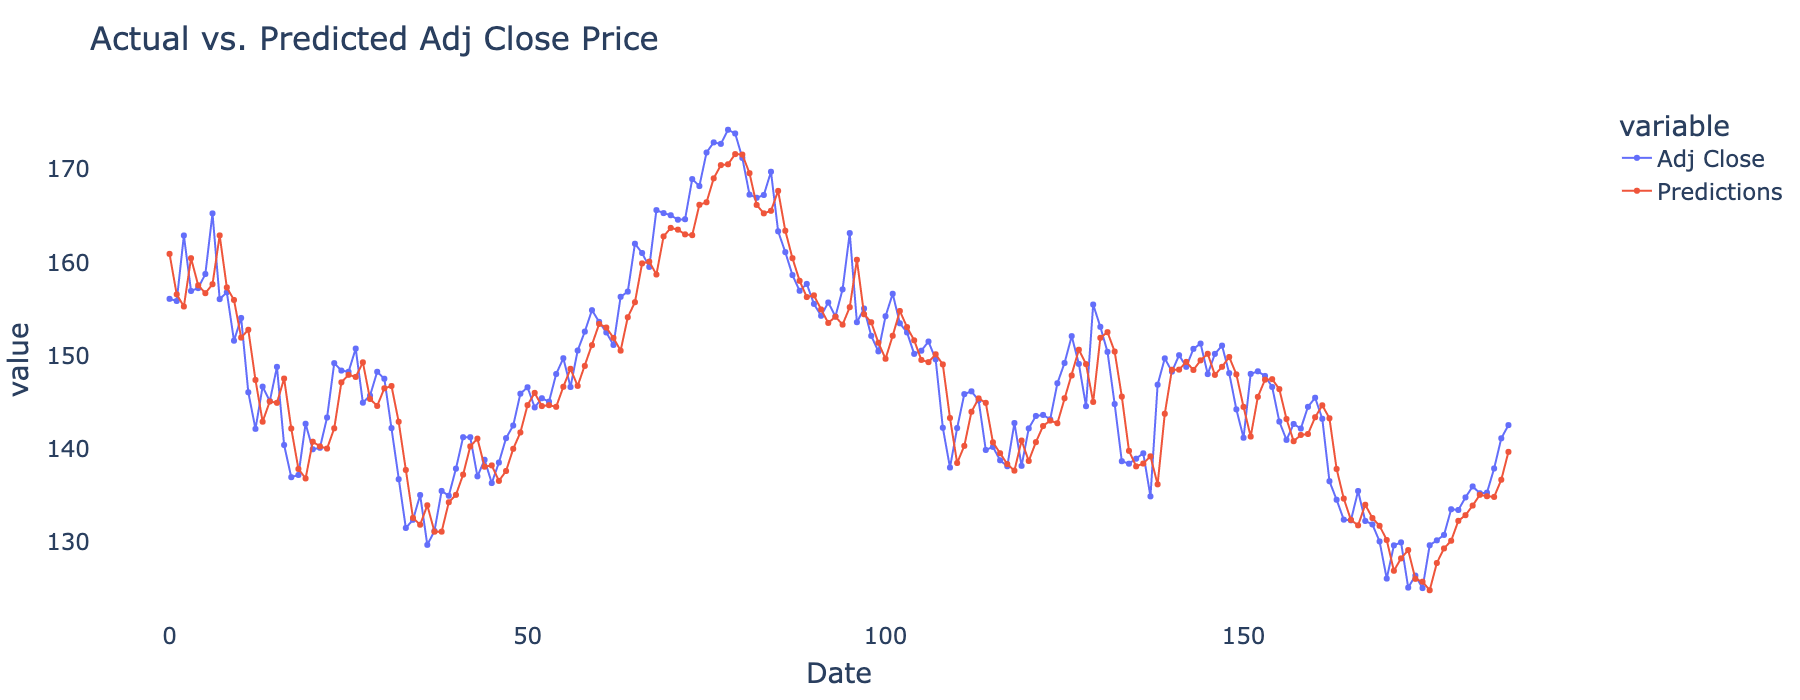
\includegraphics[width=15cm]{r1_2.png}
    \caption{Actual adjusted closing stock prices (blue) vs. adjusted closing stock prices that are predicted by the model (red)}
    \label{fig:loss2}
\end{figure}

Using six evaluation metrics—root mean squared error (RMSE), mean percentage error (MPE) mean absolute percentage error (MAPE), mean squared error (MSE),  mean absolute error (MAE), and $R^2$ score—as indicated in Table \ref{table:oa}, we make a comparison on the performance of three optimization techniques, Adam, RMSprop, and SGD. The findings indicate that while RMSprop and SGD have inferior performance with larger values for all four measures, Adam has the highest performance with the lowest values for all six metrics.

\begin{table}[!h]
\centering
\caption{Comparison of different optimization methods}
\label{table:oa}
\vspace{5pt}
\begin{tabular}{lllllll}
\thickhline
\textbf{Model} & \textbf{RMSE} & \textbf{MPE} & \textbf{MAPE} & \textbf{MSE} &\textbf{ MAE} & \textbf{$R^2$ score} \\ 
\hline
\textbf{Adam} & \textbf{3.4927} & \textbf{0.0028} & \textbf{0.0182} & \textbf{12.1992} & \textbf{2.7009} & \textbf{0.8969}\\
\hline
\textbf{RMSprop} & 3.7757 & 0.01080 & 0.0205 & 14.2565 & 3.0363 & 0.8795 \\ 
\hline
\textbf{SGD} & 8.6535 &  0.0255 & 0.0450 & 74.8843 & 6.8549 & 0.3675 \\
\thickhline
\end{tabular}

\end{table}

In a similar vein, we evaluate the effectiveness of Tanh, ReLU, and Sigmoid as three activation functions. As shown in Table \ref{table:af}, ReLU performs the best and has the lowest values for all six measures, whereas Sigmoid and Tanh perform worse and have greater values for all six metrics. 

\begin{table}[!h]
\centering
\caption{Comparison of BiLSTM with different activation functions}
\label{table:af}
\vspace{5pt}
\begin{tabular}{lllllll}
\thickhline\textbf{Model} & \textbf{RMSE} & \textbf{MPE} & \textbf{MAPE} & \textbf{MSE} &\textbf{ MAE} & \textbf{$R^2$ score} \\ 
\hline
\textbf{ReLU} & \textbf{3.4927} & \textbf{0.0028} & \textbf{0.0182} & \textbf{12.1992} & \textbf{2.7009} & \textbf{0.8969} \\
\hline
\textbf{Tanh} & 3.5385 & 0.0038 & 0.0185 & 12.5210 & 2.7445 & 0.8942 \\
\hline
\textbf{Sigmoid} & 3.6059 & -0.0005 & 0.0190 & 13.0031 & 2.8193 & 0.8901 \\
\thickhline
\end{tabular}
\end{table}

The ReLU (Rectified Linear Unit) activation function performs much better in this situation since it has the lowest values regarding all six assessment measures. 

ReLU is a particular kind of activation function that only accepts positive values and resets all negative values to zero. ReLU is hence often applied in deep learning models. It is also computationally effective and does not experience the vanishing gradients issue, which is a problem with other activation functions like the Sigmoid and Tanh.

That being said, the choice of activation function relies on the specific problem and dataset, and it's possible that the ReLU or sigmoid activation functions could work better in other contexts. It's always important to experiment with different activation functions and compare the results to find the best configuration for a particular problem.

Finally, we compare BiLSTM to other models and as can be observed in Table \ref{table:model}, BiLSTM has the lowest error score regarding all of the four performance metrics, indicating that it is the best model. 

\begin{table}[!h]
\centering
\caption{Comparison of BiLSTM and other models}
\label{table:model}
\vspace{5pt}
\begin{tabular}{lllllll}
\thickhline
\textbf{Model} & \textbf{RMSE} & \textbf{MPE} & \textbf{MAPE} & \textbf{MSE} &\textbf{ MAE} & \textbf{$R^2$ score} \\ 
\hline
\textbf{BiLSTM} & \textbf{3.4927} & \textbf{0.0028} & \textbf{0.0182} & \textbf{12.1992} & \textbf{2.7009} & \textbf{0.8969}\\
\hline
\textbf{LSTM} & 3.6231 & 0.0021 & 0.0198 & 13.1273 & 2.9242 & 0.8891 \\ 
\hline
\textbf{Vanilla RNN} & 3.6539 & 0.0062 & 0.0197 & 13.3514 & 2.9062 & 0.8872 \\
\hline
\textbf{SVR} & 43.3036 & -36.6736 & 55.3910 & 1875.2072 & 35.8522 & 0.1190 \\
\hline
\textbf{KNN} & 35.5049 & -0.4695 & 0.7507 & 1260.6012 & 23.4555 & 0.4071 \\
\thickhline
\end{tabular}
\end{table}

Table \ref{table:model} suggests that BiLSTM performs the best among the models listed, based on the evaluation metrics provided. The values of RMSE, MPE, MAPE, MSE, MAE, and $R^2$ are lowest for BiLSTM, specifically 3.4927, 0.0028, 0.0182, 12.1992, 2.7009, and 0.8969 respectively, indicating that it has the best performance, LSTM is the second-best model, followed by Vanilla RNN, SVR, and KNN.
%%%%%%%%%%%%%%%%%%%%%%%%%%%%%%%%%%%%%%%%%%%%%%%%%%%%%%%%%%%%%%%%%%%%%%%%
\section{Limitations}

In this section, we discuss one drawback of LSTM model and how Attention mechanism can be used to solve this problem through parallel computation. We then go on to discuss the problem of explainability in AI in the context of stock price prediction.
%%%%%%%%%%%%%%%%%%%%%%%%%%%%%%%%%%%%%%%%%%%%%%%%%%%%%%%%%%%%%%
\subsection{Sequential Computation}

Sequential computation is a type of computation that processes data in a sequence, one element at a time. It is in contrast to parallel computation, which processes multiple elements at the same time. Sequential computation is often used in algorithms that process data that has an inherent sequential structure, such as time series data, natural language processing, and video processing. This might be disadvantageous because:

\textbf{Training time:} BiLSTM can be computationally expensive to train, especially for large datasets or long sequences. This can make it difficult to train and deploy models in a timely manner.

\textbf{Difficulty in parallelizing:} Because BiLSTM processes data one element at a time, it can be difficult to parallelize the computation, which can limit the speed at which the model can process the data. This is solved when \cite{vaswani2017attention} proposed the use of an Attention mechanism, which allows the model to focus on particular parts of the input sequence when making a prediction, rather than processing the entire sequence as a whole. This can be particularly useful for handling long sequences, where the dependencies between elements can be very distant in the sequence.
%%%%%%%%%%%%%%%%%%%%%%%%%%%%%%%%%%%%%%%%%%%%%%%%%%%%%%%%%%%%%%
\subsection{Explainability in Artificial Intelligence (AI)}
The capacity to comprehend and analyze the justifications for judgments or predictions produced by an AI model is referred to as explainability in AI. Some drawbacks of explainability in AI when it comes to stock price prediction include:
\begin{itemize}[leftmargin=7.5pt]
    \item \textbf{Complexity:} Predicting stock prices is a difficult endeavor that requires studying a lot of data and taking into consideration a variety of variables, including economic indicators, corporate performance, and the market mood. It could be challenging to provide a clear and concise justification for the predictions provided by an AI model.
    \item \textbf{Lack of transparency:} Some AI models, such as deep learning networks, may be regarded as "black boxes" because of how demanding it is to comprehend and interpret them. Because of this lack of transparency, it may be challenging to justify the model's predictions and to increase confidence in them.
    \item \textbf{Overfitting:} Some AI models could be overfitted to the training data, which makes the model less generic to new data. The model may produce incorrect predictions as a result of overfitting, and it may be challenging to explain why.
    \item \textbf{Lack of domain expertise:} AI models could be able to evaluate a lot of data and find patterns that individuals might not be able to see. These models might not have the same degree of subject matter expertise as human analysts, and they might not completely comprehend the relevance or context of the patterns they find.
\end{itemize}
%%%%%%%%%%%%%%%%%%%%%%%%%%%%%%%%%%%%%%%%%%%%%%%%%%%%%%%%%%%%%%
\section{Conclusions}
In conclusion, Bidirectional Long Short-Term Memory (BiLSTM) - a powerful extension of Recurrent Neural Network (RNN) - is able to effectively model long-term dependencies by using gates that regulate the flow of information into and out of the cell state. Training BiLSTM to predict stock prices involves several steps, including data collection, data preprocessing, model architecture design, model training, model evaluation, model tuning, and model deployment. In this work, we show that BiLSTM works best with the Adam optimization algorithm in combination with ReLU activation function. Additionally, BiLSTM has the most outstanding performance compared to other traditional machine learning and deep learning methods. Our model is also capable of capturing complex and non-linear patterns of Apple stock prices in the five-year period.
\vfill
%%%%%%%%%%%%%%%%%%%%%%%%%%%%%%%%%%%%%%%%%%%%%%%%%%%%%%%%%%%%%%%%%%%%%%%%
\pagebreak
\nocite{*}
\bibliography{citation}
\bibliographystyle{apalike}
\end{document}
